\documentclass{article}
\usepackage{graphicx}
\usepackage{subcaption}
\usepackage{enumerate}
\usepackage{amsmath}
\DeclareMathOperator{\diag}{diag}
\usepackage{multirow}
\usepackage{booktabs}
\usepackage{bm}
\usepackage[ruled,linesnumbered]{algorithm2e}
\setcounter{MaxMatrixCols}{20}
\usepackage{tikz}
\usetikzlibrary{
  arrows.meta,
  calc,
  fit,
  positioning,
  quotes,
  graphs,
  shapes.geometric
}
\def\T{\mathrm{T}}


\title{A Greedy-based calculation method of RBS maximum allowable current}
\author{3057761608 }

\begin{document}

\maketitle

\begin{abstract}
    Reconfigurable Battery Systems (RBSs) offer a promising alternative to traditional battery systems owing to their dynamical topologic structure for the optimization of battery cell charging and discharging stragegies.
    During the operation of the RBS, the Maximum Allowable Current (MAC) is a critical indicator to guide the reconfiguring control of the system in terms of safety and reliability.
    In this paper, the MAC of the RBS is calculated by using a greedy algorithm based on the topologic model of the RBS.
    The effectiveness of this method is validated on a more complex RBS structure based on two proposed structure.
    The MAC and the computational method proposed in this article pave the way for more flexible design and more complex application scenarios, such as battery cell isolation, for RBS.


    keywords: Reconfigurable Battery System, Maximum Allowable Current, Greedy Algorithm
\end{abstract}

\section{Introduction}

Battery Energy Storage Systems (BESSs) are widely used to store and supply high-quality electrical energy in various applications, such as smart grids and wind power plants \cite{desiqueiraControlStrategySmooth2021,karandehTwoStageAlgorithmOptimal2019,yangBatteryEnergyStorage2018,choCommercialResearchBattery2015}.
Typically, a BESS consists of numerous battery cells that are interconnected by series-parallel circuitry to provide the required charge storage capacity and output voltage.
For the traditional BESS, the connections between batteries are fixed and the performance of system is limited by the worst cell, as the result of the cask effect.
Furthermore, reliability and even safety issues will alse be aroused since the failed battery cannot be promptly isolated to exacerbate the degradation of the other batteries during the operational process \cite{yangUnbalancedDischargingAging2016,fengPropagationMechanismsDiagnosis2019}.
Undoubtedly theses issues hinder the practical application of traditional BESSs.


Reconfigurable Battery System (RBS), which can dynamically switch to arbitrary circuit configurations as required, is expected to solve the above problem\cite{hanNextGenerationBatteryManagement2020a}. 
The ability to switches circuit helps to isolate unhealthy batteries from the circuit in a timely manner, thereby improving the safety and reliability of the battery system.
Fig. \ref{fig:arch} shows two popular typologies of the RBSs developed by Lawson\cite{lawsonSoftwareConfigurableBattery2012} and Visairo \cite{visairoReconfigurableBatteryPack2008} respectively. 
Taking the RBS shown in Fig. \ref{fig:arch-e} as example, the batteries in the RBS can beare connected not only in series when the switches $S_1$, $S_5$, $S_6$, $S_7$, $S_8$, $S_9$, and $S_{13}$ are closed, but also in parallel when $S_1$, $S_2$, $S_3$, $S_4$, $S_5$, $S_9$, $S_{10}$, $S_{11}$, $S_{12}$, and $S_{13}$ are closed.
Furthermore, when an unhealthy battery, for instance the orange one in Fig. \ref{fig:arch-f}, exits in the RBS, it can be isolated by closing its three adjacent switches (i.e. $S_5$, $S_7$ and $S_8$) and opening the switch below that battery (i.e. $S_6$) to ensure the system still remains a reliable working mode.

\begin{figure}[htbp]
   \centering
   \begin{subfigure}[b]{0.2\textwidth}
       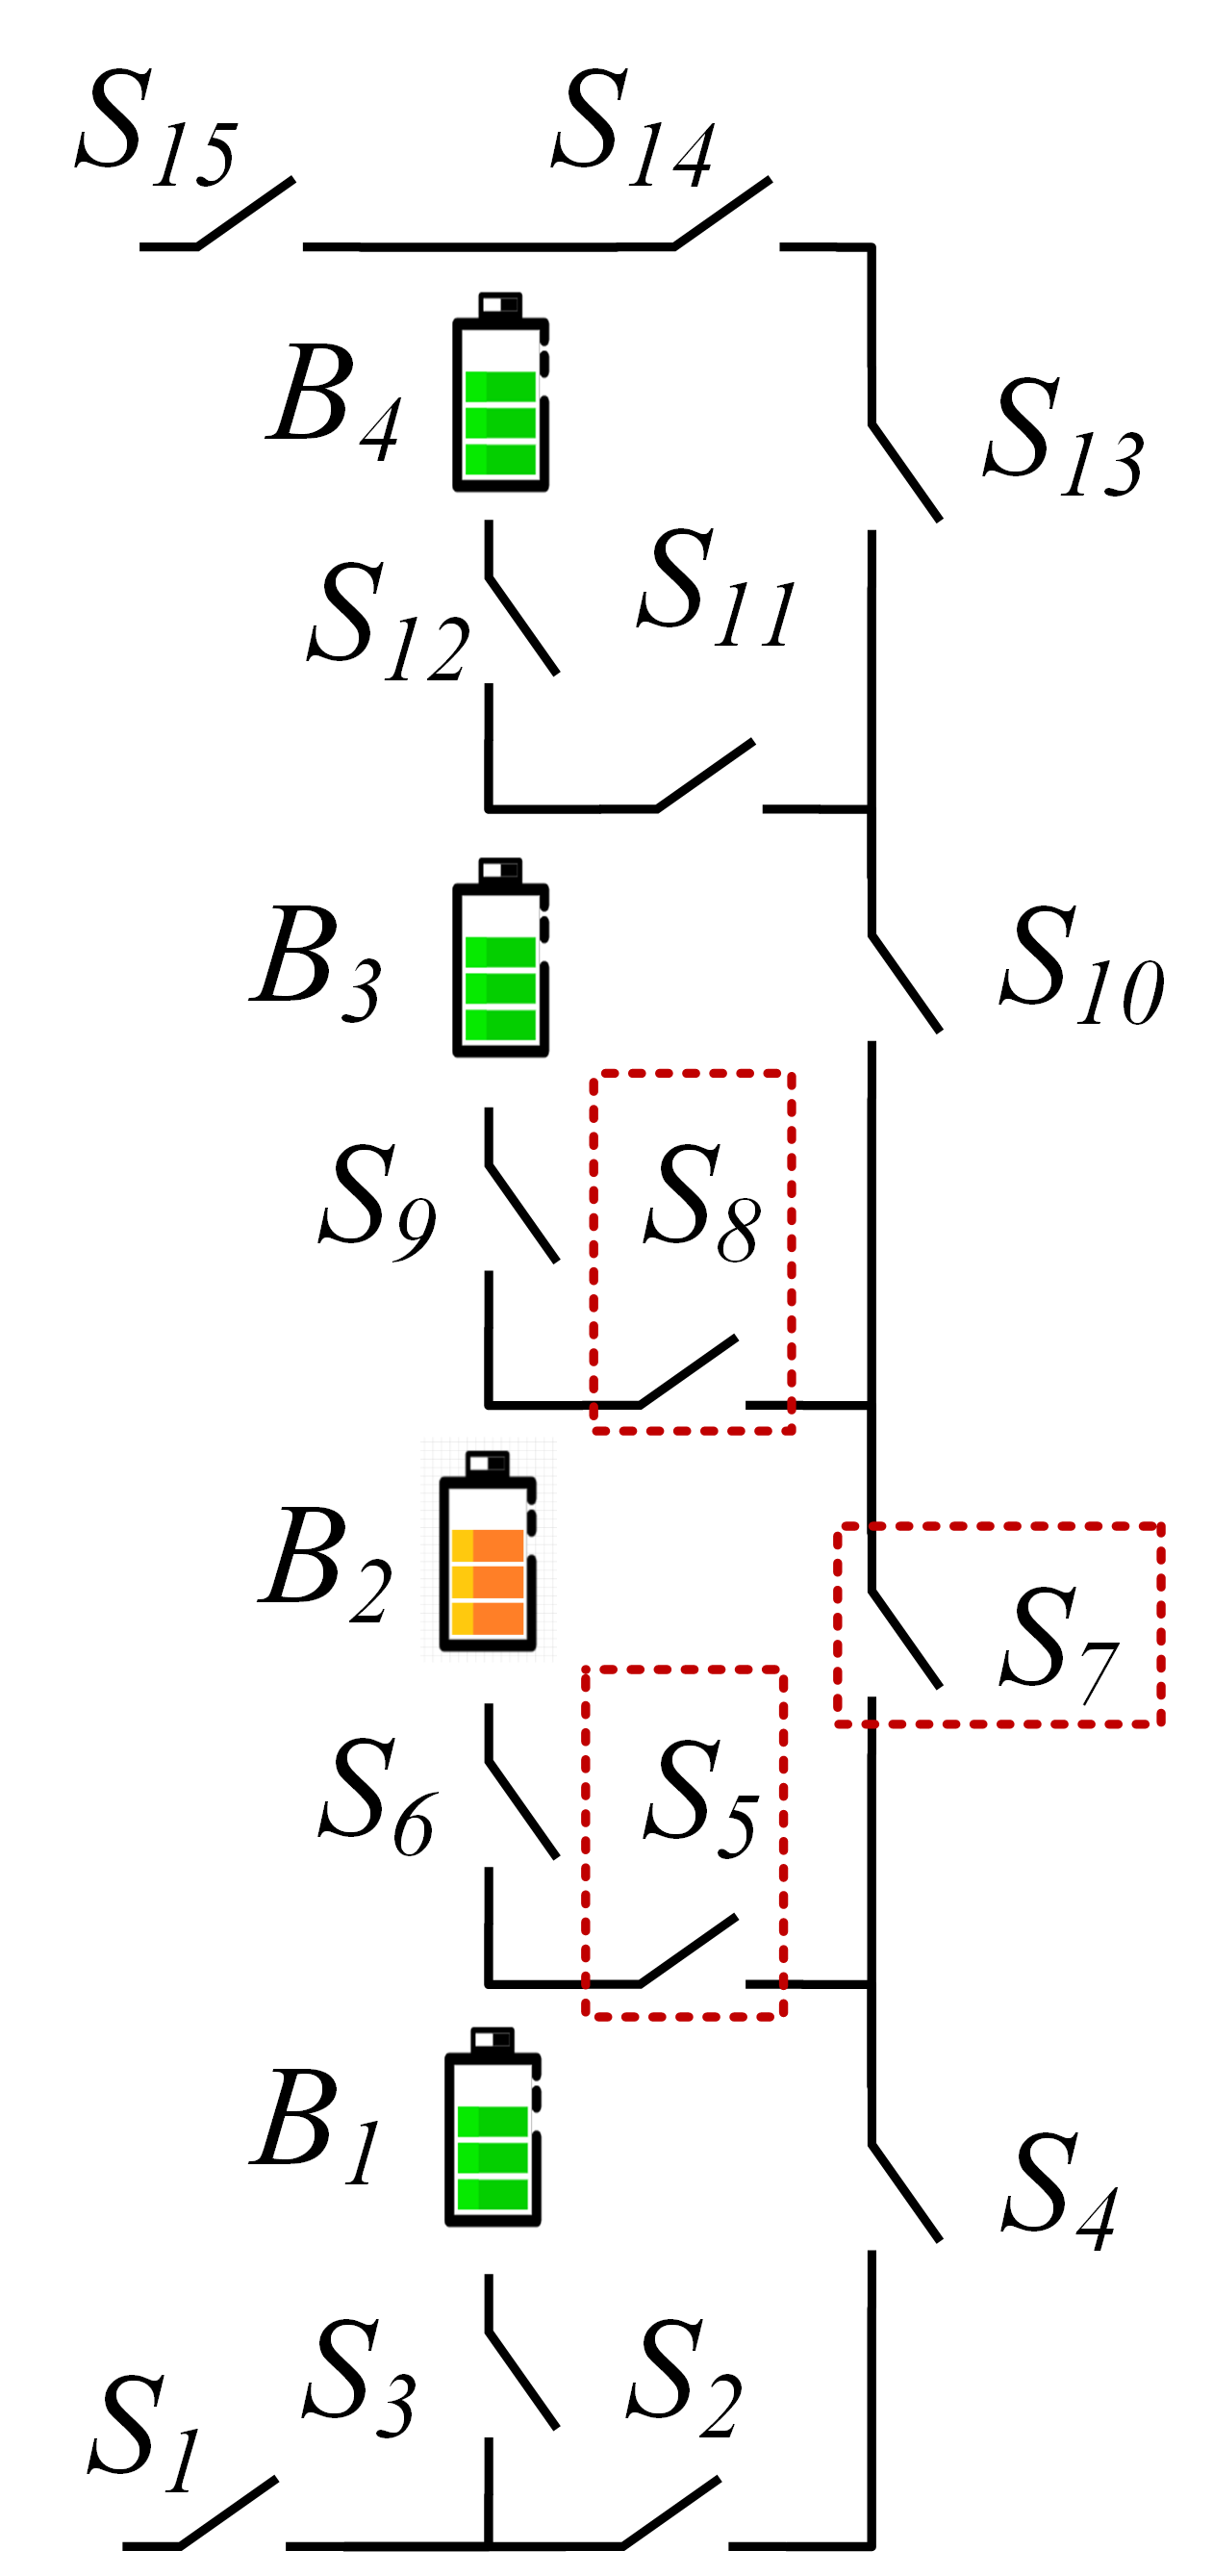
\includegraphics[width=\textwidth]{../attachments/arch-e.png}
       \caption{}
       \label{fig:arch-f}
   \end{subfigure}
   \hspace{0.05\textwidth}
   \begin{subfigure}[b]{0.45\textwidth}
       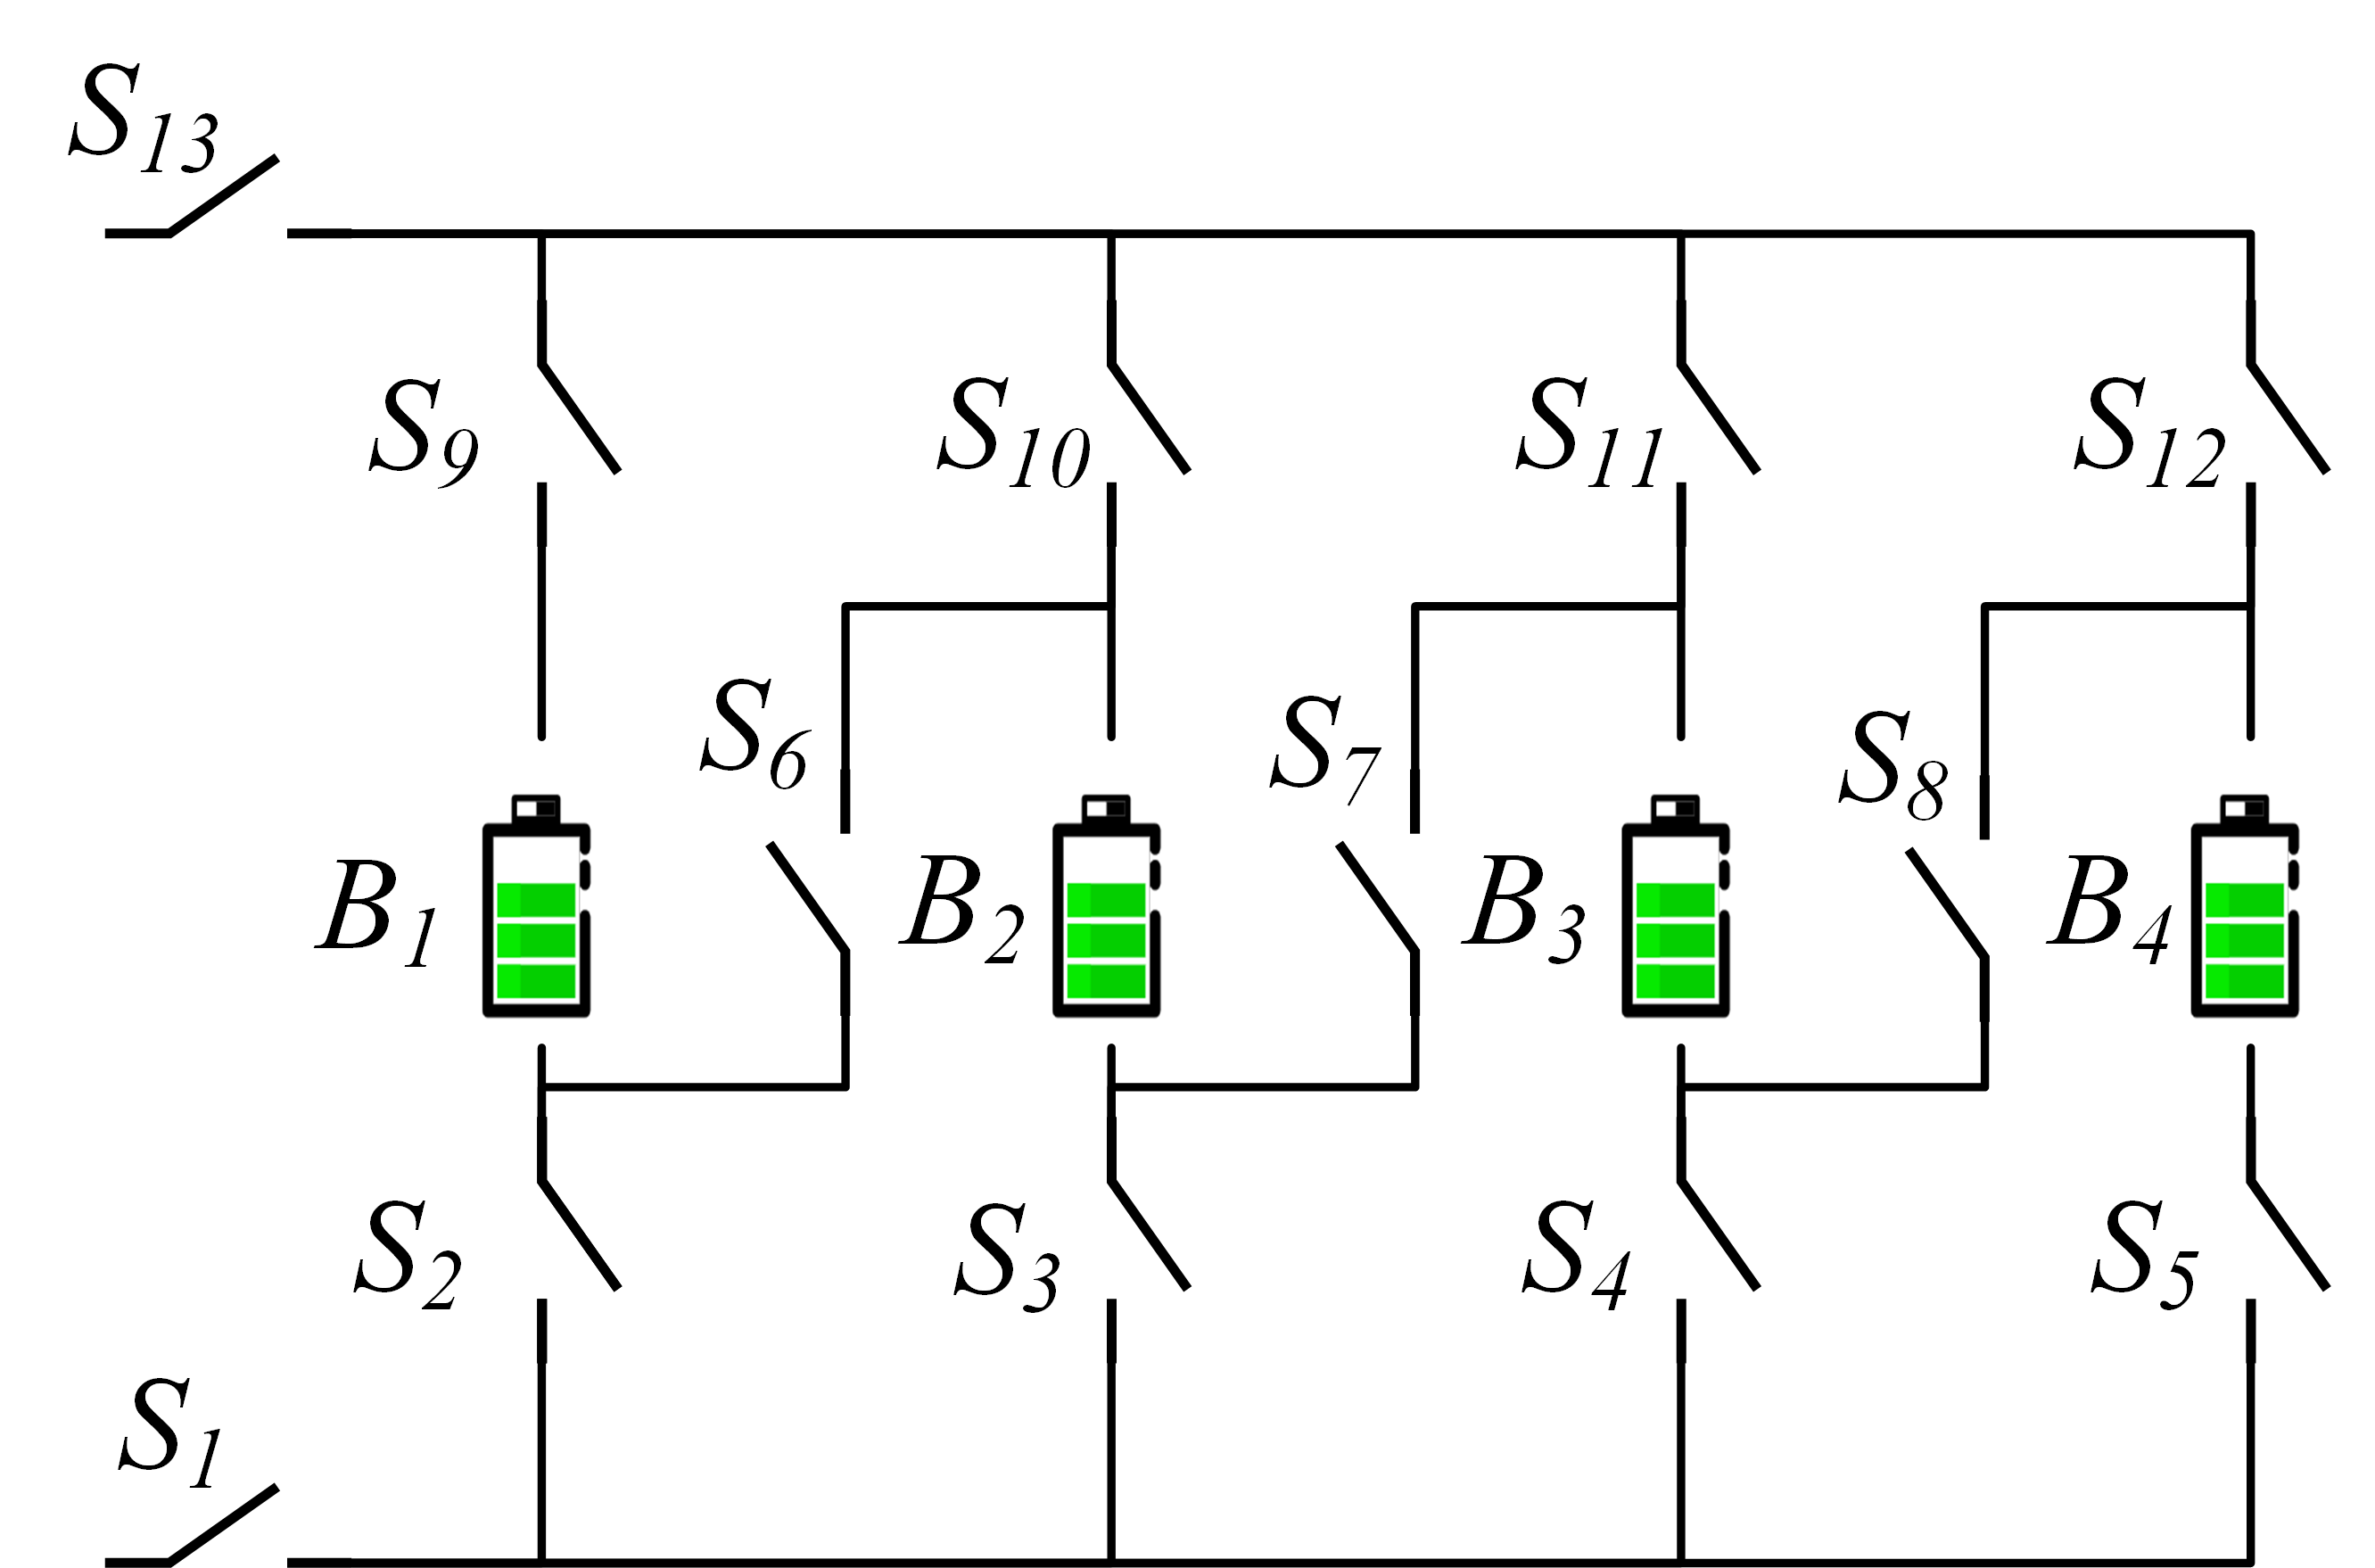
\includegraphics[width=\textwidth]{../attachments/arch-f.png}
       \caption{}
       \label{fig:arch-e}
   \end{subfigure}
    \caption{The RBS structure proposed by (a)Lawson\cite{lawsonSoftwareConfigurableBattery2012}, (b)Visairo\cite{visairoReconfigurableBatteryPack2008}.}
    \label{fig:arch}
\end{figure}

The complex connecting structure between batteries and switches enables the flexibility of the RBS, but also brings the challenges in design and control cost.
The Maximum Allowable Current (MAC) of the RBS system is defined as the maximum current that is allowed for each individual battery of the system, and is a critical indictor to be evaluate the RBS output current to the electronic appliances.
It helps the designer to assess whether the RBS meets the output current requirements, and contributes to the formulation of appropriate and safe management stragegies for the battery management system (BMS).
As the complexity of RBS increases, especially when the certain battery needs to be isolated, it becomes difficult to visually obtain the MAC, and a universal algorithm is needed to solve the MAC.
Despite its importance, there is currently no method available to evaluate MAC for RBSs.
Therefore, the purpose of this paper is to propose a universal and effective method for calculating the MAC of the RBS.
To achieve this, a topologic model that builds the relationship between RBS circuit topology and internal resistance and voltage of its batteries are established.
Then, a greedy algorithm is employed to search the available circuit of the RBS for reaching the MAC.
With the developed method, MAC of RBSs with different structures can be calculated effectively, including application scenarios with isolated battery cells.


The remainder of this paper is organized as follows:
Section II presents the framework and details of the proposed topologic model and the greedy algorithm.
In Section III, a case study of using the proposed model and algorithm to enumerate the MAC of a new and complex structure is demonstrated.
The calculation results and scenarios such as battery cells isolation also are discussed
Finally, the concluding remarks are drawn in Section IV.


\section{Methodology}

The overall MAC modeling process from an RBS structure is shown in Fig. \ref{fig:main}, which can be divided into four main steps.
In the first place, the actual RBS structure is converted to a topologic model, in which the connected relationships between batteries and switches are abstracted and the performance parameters of the batteries are retained.
Subsequently, constraints and objective function, i.e. MAC, are obtained based on the previous connected relationships and parameters.
Then, the shortest path (SP) of each battery in the RBS is obtained by Dijkstra algorithm.
In the end, the open/close strategy of the RBS is implemented by greedily selecting the SPs to achieve MAC and quantitatively calculated in the equivalent circuit.

\begin{figure}[htbp]
    \centering
    \begin{subfigure}[b]{\textwidth}
        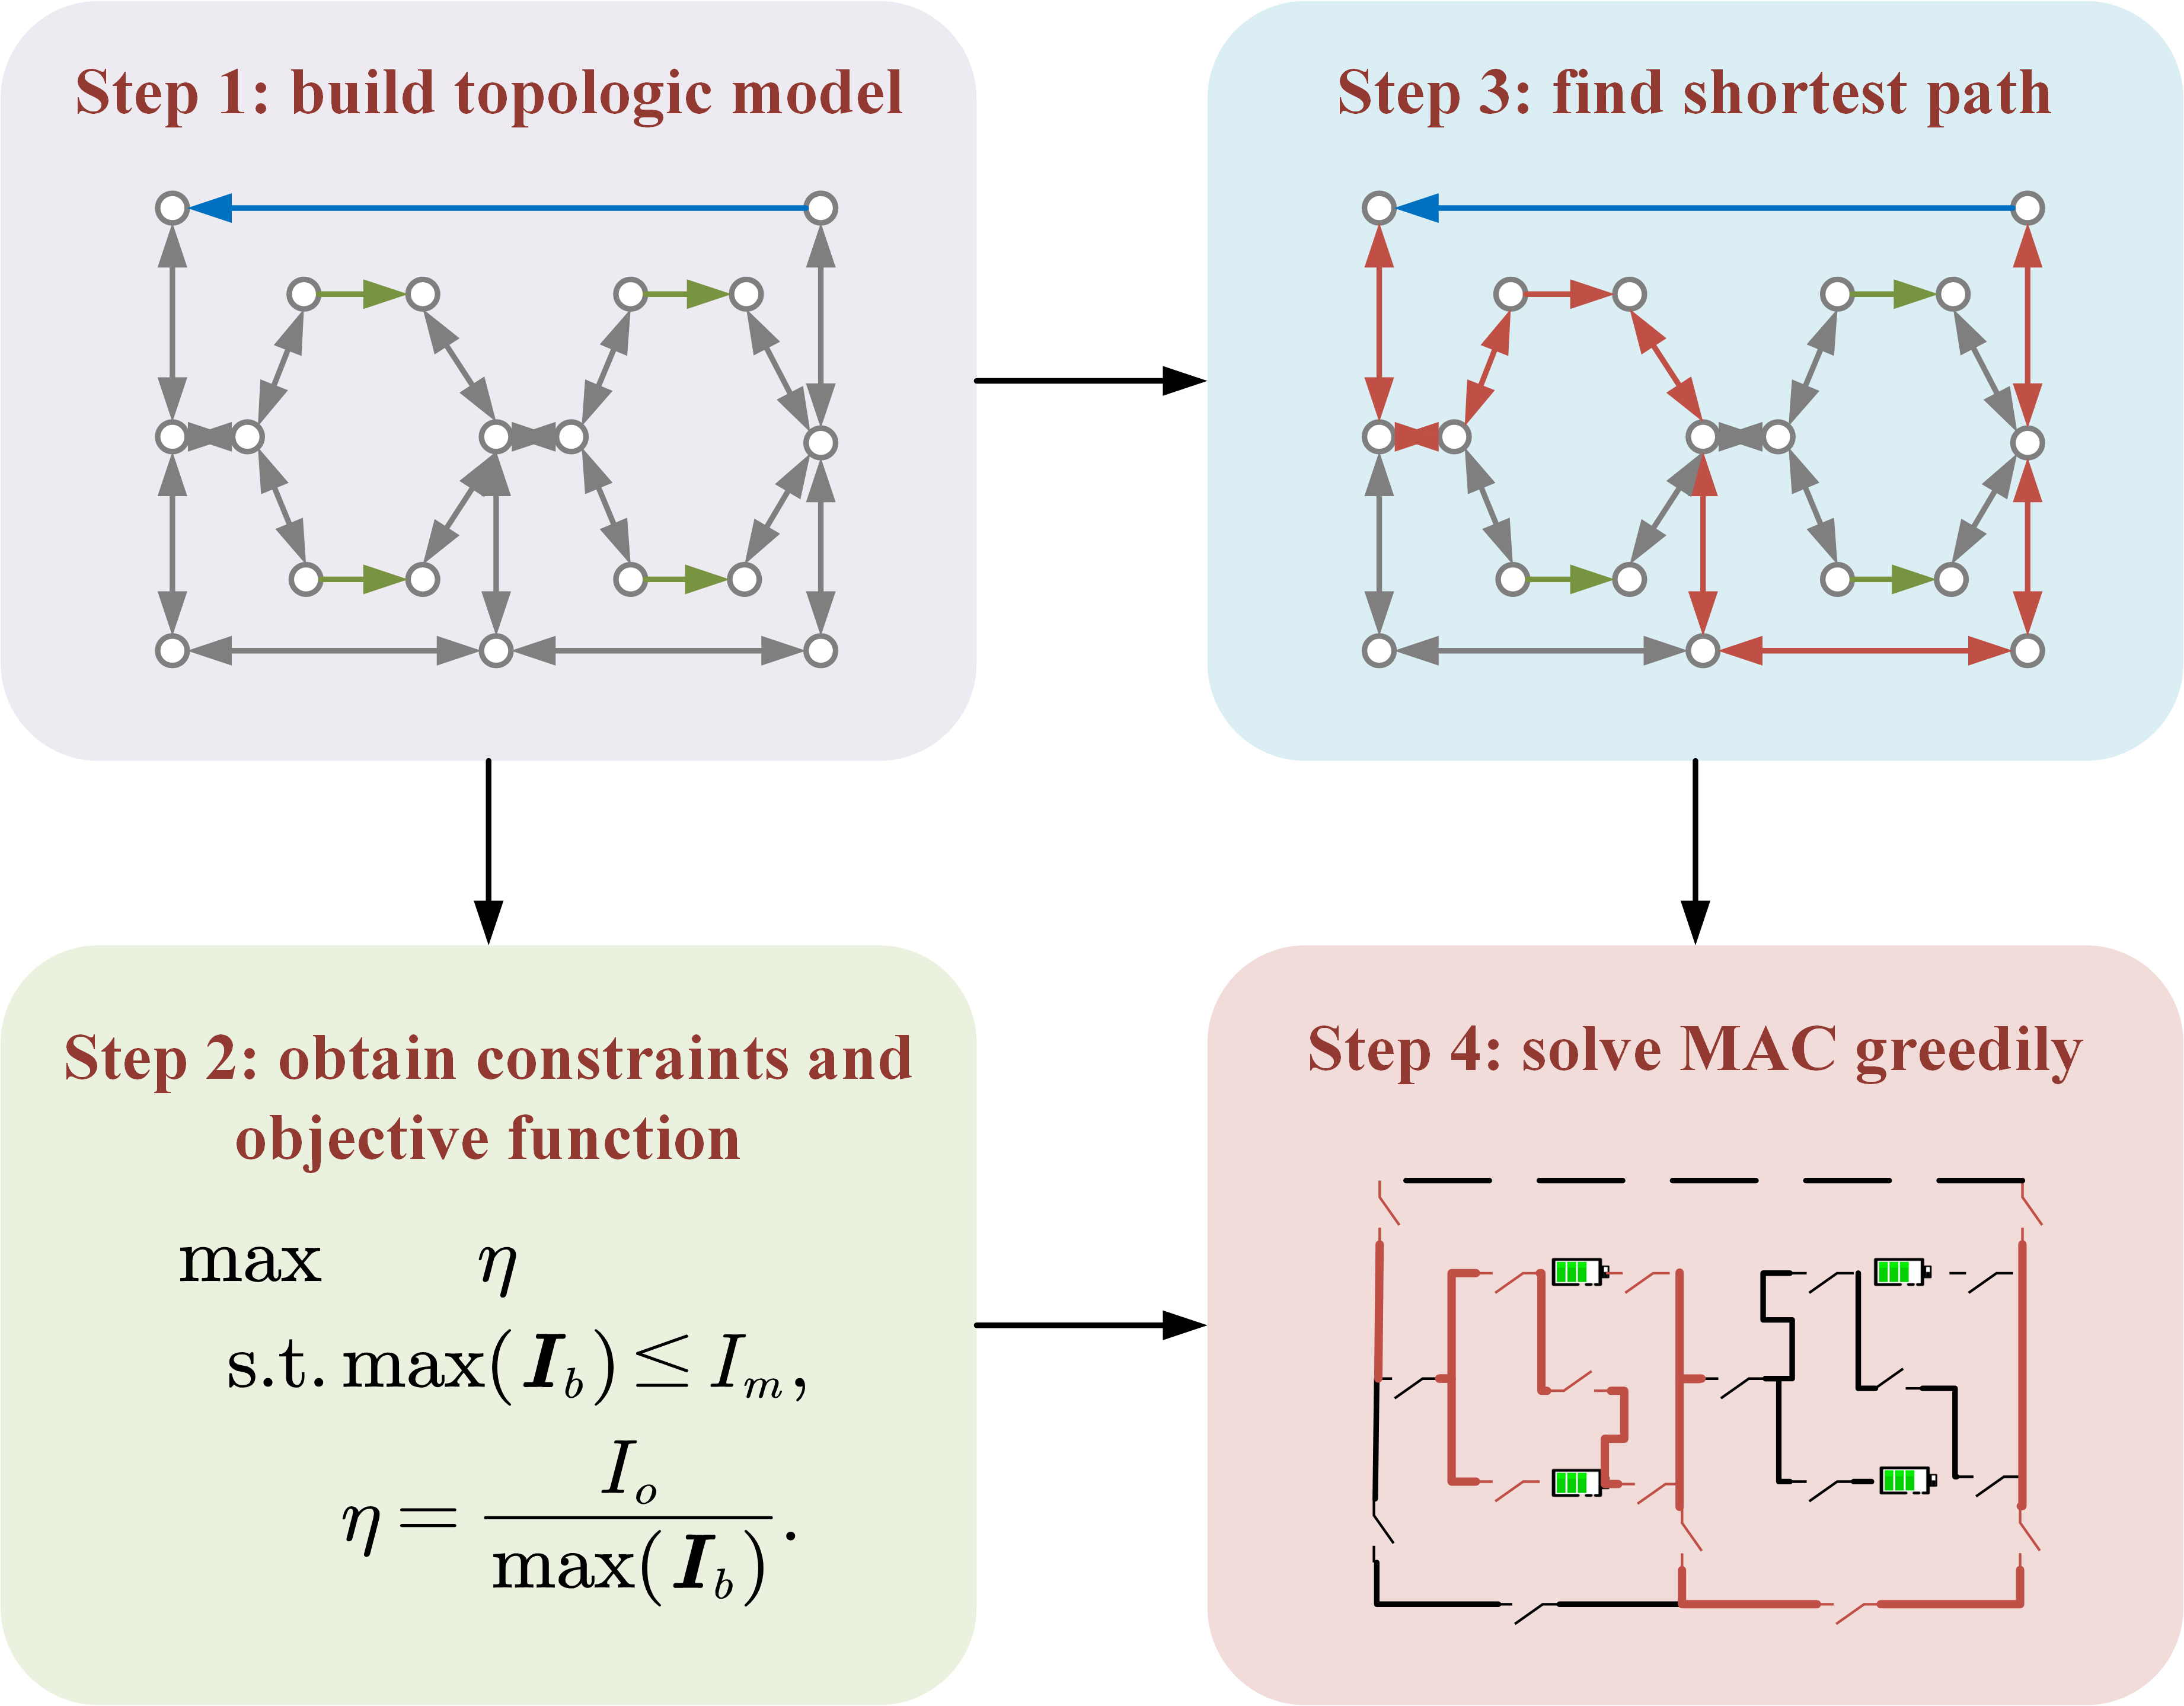
\includegraphics[width=\textwidth]{../attachments/main.png}
        \caption{}
        \label{fig:main}
    \end{subfigure}
    \\ 
    \begin{subfigure}[b]{\textwidth}
        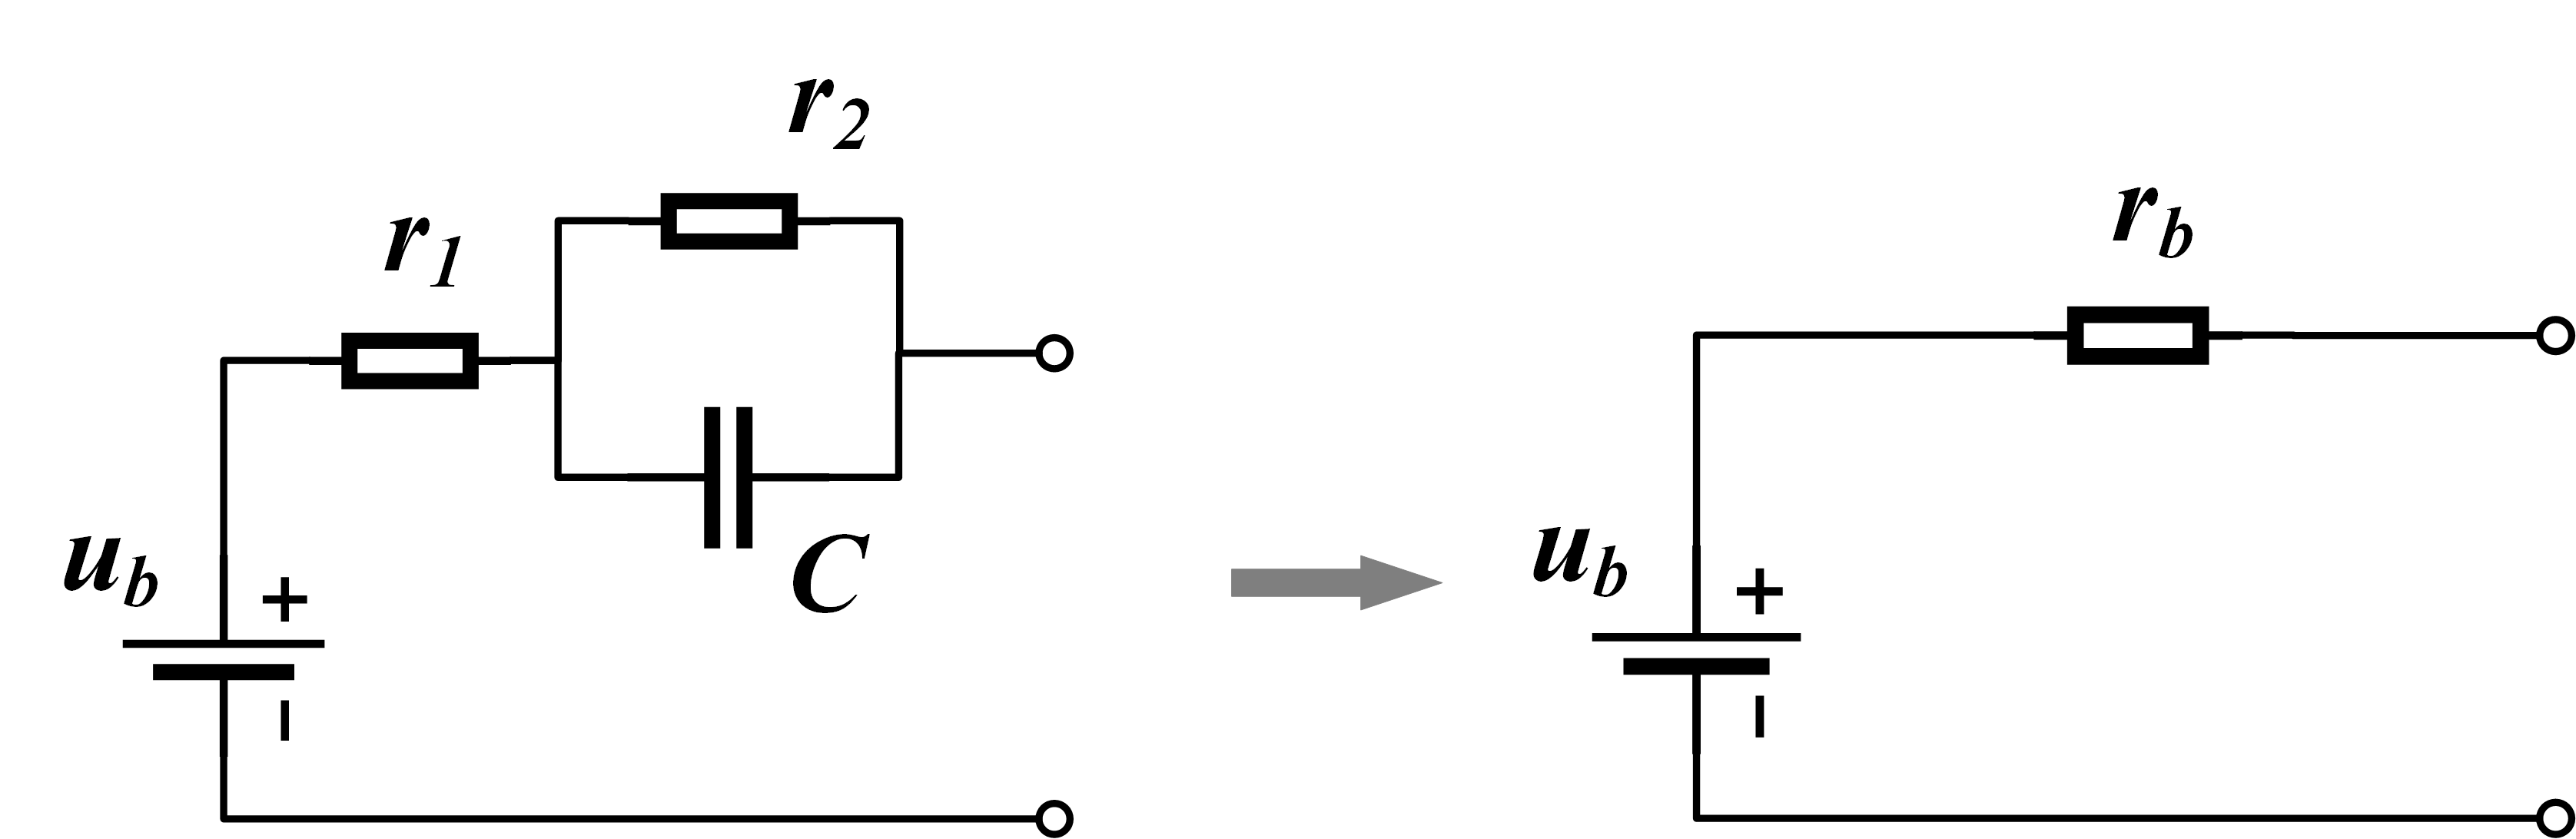
\includegraphics[width=\textwidth]{../attachments/battery_simple.png}
        \caption{}
        \label{fig:battery_simple}
    \end{subfigure}
    \caption{(a)Diagram of this method, which contains four main steps.
    Step 1: The RBS structure is converted to a topologic model.
    Step 2: Constraints and objective function are obtained based on the previous topologic model.
    Step 3: The shortest path of each battery in the RBS is obtained by Dijkstra algorithm.
    Step 4: The MAC is achieved by greedily selecting the shortest paths to open/close switches.
    (b) The equivalent circuit of a battery in this method, with $u_{b,i}$ and $r_{b,i}$ representing the voltage and internal resistance of the battery $i$ respectively.
    The capacitor in Thevenin model is ignored.
    }
\end{figure}

\subsection{Topologic Model}

As demonstrated in Fig. \ref{fig:arch}, a typical RBS is made up of a number of battery cells and switches in a dynamically adjustable connection.
To establish a processable circuit, these batteries and switches are transformed into ideal elements under reasonable assumptions.
The resulting circuit structure is then described in matrix form, and the related equations are provided.


The normal equivalent circuit for a battery consists of a voltage source in series with a resistor, and a capacitor in parallel with another resistor to simulate the polarization in batteries, kwon as Thevenin model\cite{hongwenheStateofChargeEstimationLithiumIon2011,mousavig.VariousBatteryModels2014}.
To simplify the model, the transient characteristics of the circuit are not considered, so the capacitor mentioned above is ignored.
In this way, the battery $i$ in the RBS is modeled by the series connection in between a constant voltage source $u_{b,i}$ and a resistor $r_{b,i}$,  as shown in Fig. \ref{fig:battery_simple}
And a binary variable $x_j$ is used to represent the state of switch $j$, where 0 for ON and 1 for OFF, respectively.
To simplify the calculation, a closed switch is considered as a resistor with a very small resistance value $r_s$.


For a given RBS structure, the topologic model for the RBS is constructed as a directed graph $G(V,E)$ in such a way that:
\begin{enumerate}
    \item Nodes: node $v_1$ and $v_N$ represent the anode and cathode of the RBS respectively, and the other nodes $v_2,\cdots , v_{N-1}$ represent the points connecting batteries and/or switches, where $N$ is the total number of nodes.
    \item Edges: the directed edges represent batteries, switches and the external electrical appliance in the output circuit based on whether the current direction is constrainted or not. 
        When the battery is in operation, the internal current direction must be from the negative electrode to the positive electrode, so it is represented by a directed edge from the negative to the positive ; this edge has attributes $(u_b, r_b)$, where $u_b$ and $r_b$ represent battery $b$'s electromotive force and internal resistance.
        Switches have no constraints on the current direction, so they are represented by a pair of directed edges with opposite directions; these edges both have attribute $(0, r_s)$, where $r_s$ represents the resistance of switch as mentioned above.
        To fully solve for the current and voltage, an external electrical appliance equivalent as a resistor $R_0$ is connected to the anode and cathode of the RBS and represented by a directed edge from the anode $v_N$  to the cathode $v_1$ of the RBS.
        Similarly, this edge has attribute $(0, R_0)$.
        If a given RBS structure has $N_b$ batteries and $N_s$ switches in total, then the number of edges is $N_b+2N_s+1$, where 1 refers to the external electrical appliance.
\end{enumerate}

\subsection{Constraints and Objective Function}

The constraints and objective function are obtained by analyzing the currents of batteries and external electrical appliance, as following.
Based on the above directed graph which has $N$ nodes and $N_b+2N_s+1$ directed edges, its incidence matrix $\bm{A}$ is defined as
\begin{align}\label{eq:A}
    a_{ij}=
    \begin{cases}
        1,  & \text{edge  $j$ leaves vertex $i$},\\
        -1, & \text{edge $j$ enters vertex $i$},\\
        0,  & \text{otherwise}.
    \end{cases}
\end{align}
Since each column of $\bm{A}$ sums to zero, the last line are deleted.
Furthermore, because of a couple of opposite directed edges for each switch, the $N_s$ columns corresponding to the switches are also deleted.
Finally, the reduced incidence matrix $\bm{A}_{(N-1)\times(N_b+N_s+1)}$ are used in the following calculation.
By divided as batteries, switches and external electrical appliance, $A$ is rewritten as follows
\begin{equation}
    \bm{A} =
    \begin{bmatrix}
        \bm{A}_b & \bm{A}_s & \bm{A}_o
    \end{bmatrix}.
\end{equation}


$N_b+N_s+1$ edges' currents $\bm{I}_{(N_b+N_s+1)\times 1}$ and voltages $\bm{U}_{(N_b+N_s+1)\times 1}$, and $N-1$ nodes' voltages $\bm{U}_{n, (N-1)\times 1}$ have following relationships from Kirchhoffs law
\begin{align}\label{eq:Kirchhoffs_law}
    \begin{cases}
        \bm{A} \bm{I} = \bm{0}, \\
        \bm{U}        = \bm{A}^\T \bm{U}_n.
    \end{cases}
\end{align}
These directed edges are treated as generalized branches and expressed in matrix form as follows
\begin{equation}\label{eq:generalized_branches}
    \bm{I} = \bm{Y}\bm{X} \bm{U} - \bm{Y}\bm{X} \bm{U}_s +\bm{I}_s,
\end{equation}
where $\bm{I}$ and $\bm{U}$ are the column vectors about $1+N_b+N_s$ edges' current and voltage, respectively;
$\bm{U}_s$ and $\bm{I}_s$ denote the source voltage and source current of the generalized branches, respectively;
$\bm{Y}$ is the admittance matrix of the circuit, and $\bm{X}$ is the state matrix defined as
\begin{equation}\label{eq:X}
    \bm{X} = \diag(
    \underbrace{1, \cdots, 1}_{N_b~\text{of}~1},
    \underbrace{1, 0 \cdots, 1}_{N_s~\text{of}~0/1},
    1)
    =\begin{bmatrix}
        \bm{I} & & \\
        & \bm{X}_s &\\
        & &\bm{I}
    \end{bmatrix}.
\end{equation}


In addition to the equivalent circuit assumptions, we also assume that all batteries have the same internal resistance value $r_b$ and supply the same electric potential $u_s$ to simplify the model.
Then the output current $I_o$ and each battery's current $\bm{I}_b$ can be given by solving the simultaneous Eq. \ref{eq:Kirchhoffs_law} and \ref{eq:generalized_branches} eventually.
Let
\begin{equation}\label{eq:Yn}
    \bm{Y}_n (\bm{X}_s) = \frac{1}{R_o} \bm{A}_o\bm{A}_o^\T + \frac{1}{r_b} \bm{A}_b\bm{A}_b^\T + \frac{1}{r_s}\bm{A}_s\bm{X}_s\bm{A}_s^\T,
\end{equation}
where $R_o$ is the equivalent resistance of the external circuit.
Then, if $\bm{Y}_n$ is an invertible matrix,
\begin{equation}
    I_o(\bm{X}_s)       = \frac{u_b}{R_o r_b} \bm{A}_o^\T \bm{Y}_n^{-1}(\bm{X}) \bm{A}_b \bm{I}_{N_b\times 1};\label{eq:I_o}
\end{equation}
\begin{equation}
    \bm{I}_b(\bm{X}_s)  = \frac{u_b}{r_b^2}[\bm{A}_b^\T \bm{Y}_n^{-1}(\bm{X}) \bm{A}_b\bm{I}_{N_b \times 1}  -r_b \bm{I}_{N_b \times 1}],\label{eq:I_b}
\end{equation}
where $\bm{I}_{N_b\times 1}$ is a column vector with all equal to 1.


In this study, the ratio of $I_o$ and $\max (\bm{I}_b)$ is used to characterize the maximum allowable current for a given RBS architecture, denoted as $\eta$:
\begin{equation}\label{eq:eta}
    \eta = \frac{I_o}{\max (\bm{I}_b)}.
\end{equation}
The discussion in the next section will show that the $\eta$ reflects the ability of the RBS architecture itself to deliver current, regardliess of the battery cells used by the RBS.
Finally the problem in RBS can be formulated as
\begin{align}
    & \max \eta \label{eq:max_eta}\\
    \text{s.t.} & \max (\bm{I}_b) \leq I_m, \label{eq:Ib_leq_Im}
\end{align}
where $I_m$ is the maximum allowable current of the battery; $\eta$ can be calculated by Eq. \ref{eq:eta}; $I_o$ and $\bm{I}_b$ can be calculated by Eq. \ref{eq:I_o} and \ref{eq:I_b}.
However, it is computationally difficult to solve Eq. \ref{eq:max_eta} directly because of the presence of matrix $\bm{Y}_n^{-1}$.
As the number of batteries and switches in the RBS increase, the order of the matrix increases, and the time costed to compute increases sharply.
A greedy algorithm will be proposed to solve this problem in the next subsection.


The integrability of the matrix $\bm{Y}_n$ is explained here.
Although the above solution procedure requires the matrix $\bm{Y}_n$ to be invertible, it is still possible to encounter integrable $\bm{Y}_n$ in the calculation.
The physical meaning of this case corresponds to the fact that due to the excessive number of switches in OFF, the solved circuit structure forms circuit branches independent of the main circuit, i.e., the circuit connected to the anode and cathode of the RBS. 
Since these independent branches are not connected to the main circuit, the voltage potentials of these branches cannot be determined and theoretically an infinite number of sets of solutions exist. 
Benfit from the independence, these solutions have no influence on the results of the main circuit. 
Since only the currents and voltages of the main circuit are of interest, only one of these solutions needs to be chosen for subsequent calculation.

\subsection{Greedy Solution}\label{subsec:greedy_solution}

In this subsection, a greedy algorithm is proposed based on shortest paths ($SP$s), which is given here firstly.
When the battery $i$ is connected to the anode $v_1$ and the cathode $v_N$ of the RBS by the path $p$ in the graph model, the distance $\omega$ of $p$ is defined by the following equation:
\begin{equation}\label{eq:weight}
    \omega(p) = N_s \cdot n_b (p) + n_s (p),
\end{equation}
where $N_s$ is the total number of switches in the system; $n_b(p)$ and $n_s(p)$ are number of batteries and switches in the path $p$ respectively.
$SP_i$ is defined as the path with the minimum $\omega$ for battery $i$.
\begin{equation}\label{eq:def_sp}
    SP_i = \mathop{\arg\min}_{p \in P_i} \omega(p),
\end{equation}
where $P_i$ is the set of all paths from $v_1$ to $v_N$ and passed through the directed edge $i$ in the direction of it.
Specifically, the Dijkstra algorithm can be used to implement the $SP_i$.
According to the definition, $SP_i$ gives the simplest strategy by which the control of battery $i$ is achieved with a minimum of switches while minimizing the influence of other batteries.
From the perspective of series/parallel, the more batteries are connected into circuit via their $SP$s, the more batteries are connected in parallel.
Since batteries can provide more total output current when connected in parallel than in series, the algorithm greedily selects as many cells as possible to be connected into to the overall circuit via their $SP$s to obtain the MAC.
The dichotomy method is also performed to faster find the right number of $SP$s.

After finding the potential SPs combinations about the MAC, the state variable $\bm{X}_s$ of the switches can be determined, and the optimization problem \ref{eq:max_eta} can be solved using Eq. \ref{eq:eta}, \ref{eq:I_o} and \ref{eq:I_b}.
The overall flowchart is shown in Fig. \ref{fig:flowchart}, and the corresponding pseudo-code of the algorithm is shown in Algorithm \ref{alg:eta_RBS}.

\tikzset{
  meta box/.style={
    draw,
    black,
    very thick,
    text centered,
  },
  punkt/.style={
    meta box,
    rectangle,
    rounded corners,
    inner sep=.25em,
    minimum height=2em,
    minimum width=4em,
    align=center,
    text width=10em
  },
  round/.style={
    meta box,
    circle,
    minimum size=0,
    inner sep=0pt, 
    outer sep=0pt
  },
  every fit/.style={
    draw,
    thick,
    dashed,
    gray,
    inner xsep=.5em,
    inner ysep=.75em
  }
}
\begin{figure}
% \begin{tikzpicture}[font=\small, node font=\small, node distance=1.5em]
%     \node[punkt]     (input) {Input: RBS structure};
%     \node[punkt, below=0.3of input] (get_SP) {get $SP$s by Eqs. \ref{eq:weight} and \ref{eq:def_sp} and Dijkstra Search};
%     \node[punkt, below=0.3of get_SP] (get_A) {get $\bm{A}$ from Eq. \ref{eq:A}};
%     \node[punkt, below=0.3of get_A] (get_Nset) {init $N_{set}=N_b$ };
%     \node[punkt, below=0.3of get_Nset] (get_cb) {get $c_b$s by combinating $N_{set}$ batteries from $N_b$};
%     \node[draw, diamond, aspect=2, below=0.3of get_cb] (is_check_all_cb) {are all $c_b$s checked?};
%     \node[draw, diamond, aspect=2, right=1of is_check_all_cb] (is_Nset_converged) {is $N_{set}$ converged?};
%     \node[punkt, above=of is_Nset_converged] (reset_Nset) {reset $N_{set}$ by dichotomy};
%     \node[punkt, text width=15em, below=0.3of is_check_all_cb] (get_Xs) {
%         select an unchecked $c_b$, and get its $\bm{X}_m$ by \\ 
%         if switch $j$ $\in \bigcup_{i\in c_b}SP_i$:\\
%         $\bm{X}[j]=1$ else $0$};
%     \node[punkt, below=0.3of get_Xs] (get_Yn) {get $\bm{Y}_n$ by Eq.\ref{eq:Yn}};
%     \node[draw, diamond, aspect=2, below=0.3of get_Yn] (is_Yn_invertible) {is $\bm{Y}_n$ invertible?};
%     \node[punkt, right=1.3of is_Yn_invertible] (construct) {construct an effective solution};
%     \node[punkt, below=0.3of is_Yn_invertible] (get_I) {get $I_o$ and $\bm{I}_b$ by Eqs. \ref{eq:I_o} and \ref{eq:I_b}};
%     \node[draw, diamond, aspect=2, below=0.3of get_I] (is_leq_Im) {is $\max \bm{I}_b \leq I_m$?};
%     \node[punkt, right=1.3of is_leq_Im] (drop_eta) {drop this $\eta$};
%     \node[punkt, below=0.3of is_leq_Im] (get_eta) {get $\eta$ by Eq.\ref{eq:eta}};
%     \node[punkt, below=0.3of get_eta] (update_max_eta) {update $\max \eta$};
%     \node[punkt, right=1of is_Nset_converged] (output) {Output: $\max \eta$};
%     \node[round,left=1.5of update_max_eta](point1){};
% 
%     \graph{
%       (input) -> (get_SP) -> (get_A) -> (get_Nset) -> (get_cb) -> (is_check_all_cb) ->["No"] (get_Xs) -> (get_Yn) -> (is_Yn_invertible) ->["Yes"] (get_I) -> (is_leq_Im) ->["Yes"] (get_eta) -> (update_max_eta);
%       (is_check_all_cb) ->["Yes"] (is_Nset_converged) ->["No"] (reset_Nset) -> (get_cb);
%       (is_Yn_invertible) ->["No"] (construct) ->[to path={|- (\tikztotarget)}] (get_I);
%       (is_leq_Im) ->["No"] (drop_eta) ->[to path={|- (\tikztotarget)}] (update_max_eta);
%       (is_Nset_converged) ->["Yes"] (output);
%       (update_max_eta) -- (point1) ->[to path={|- (\tikztotarget)}] (is_check_all_cb);
%     };
% \end{tikzpicture}
    \centering
    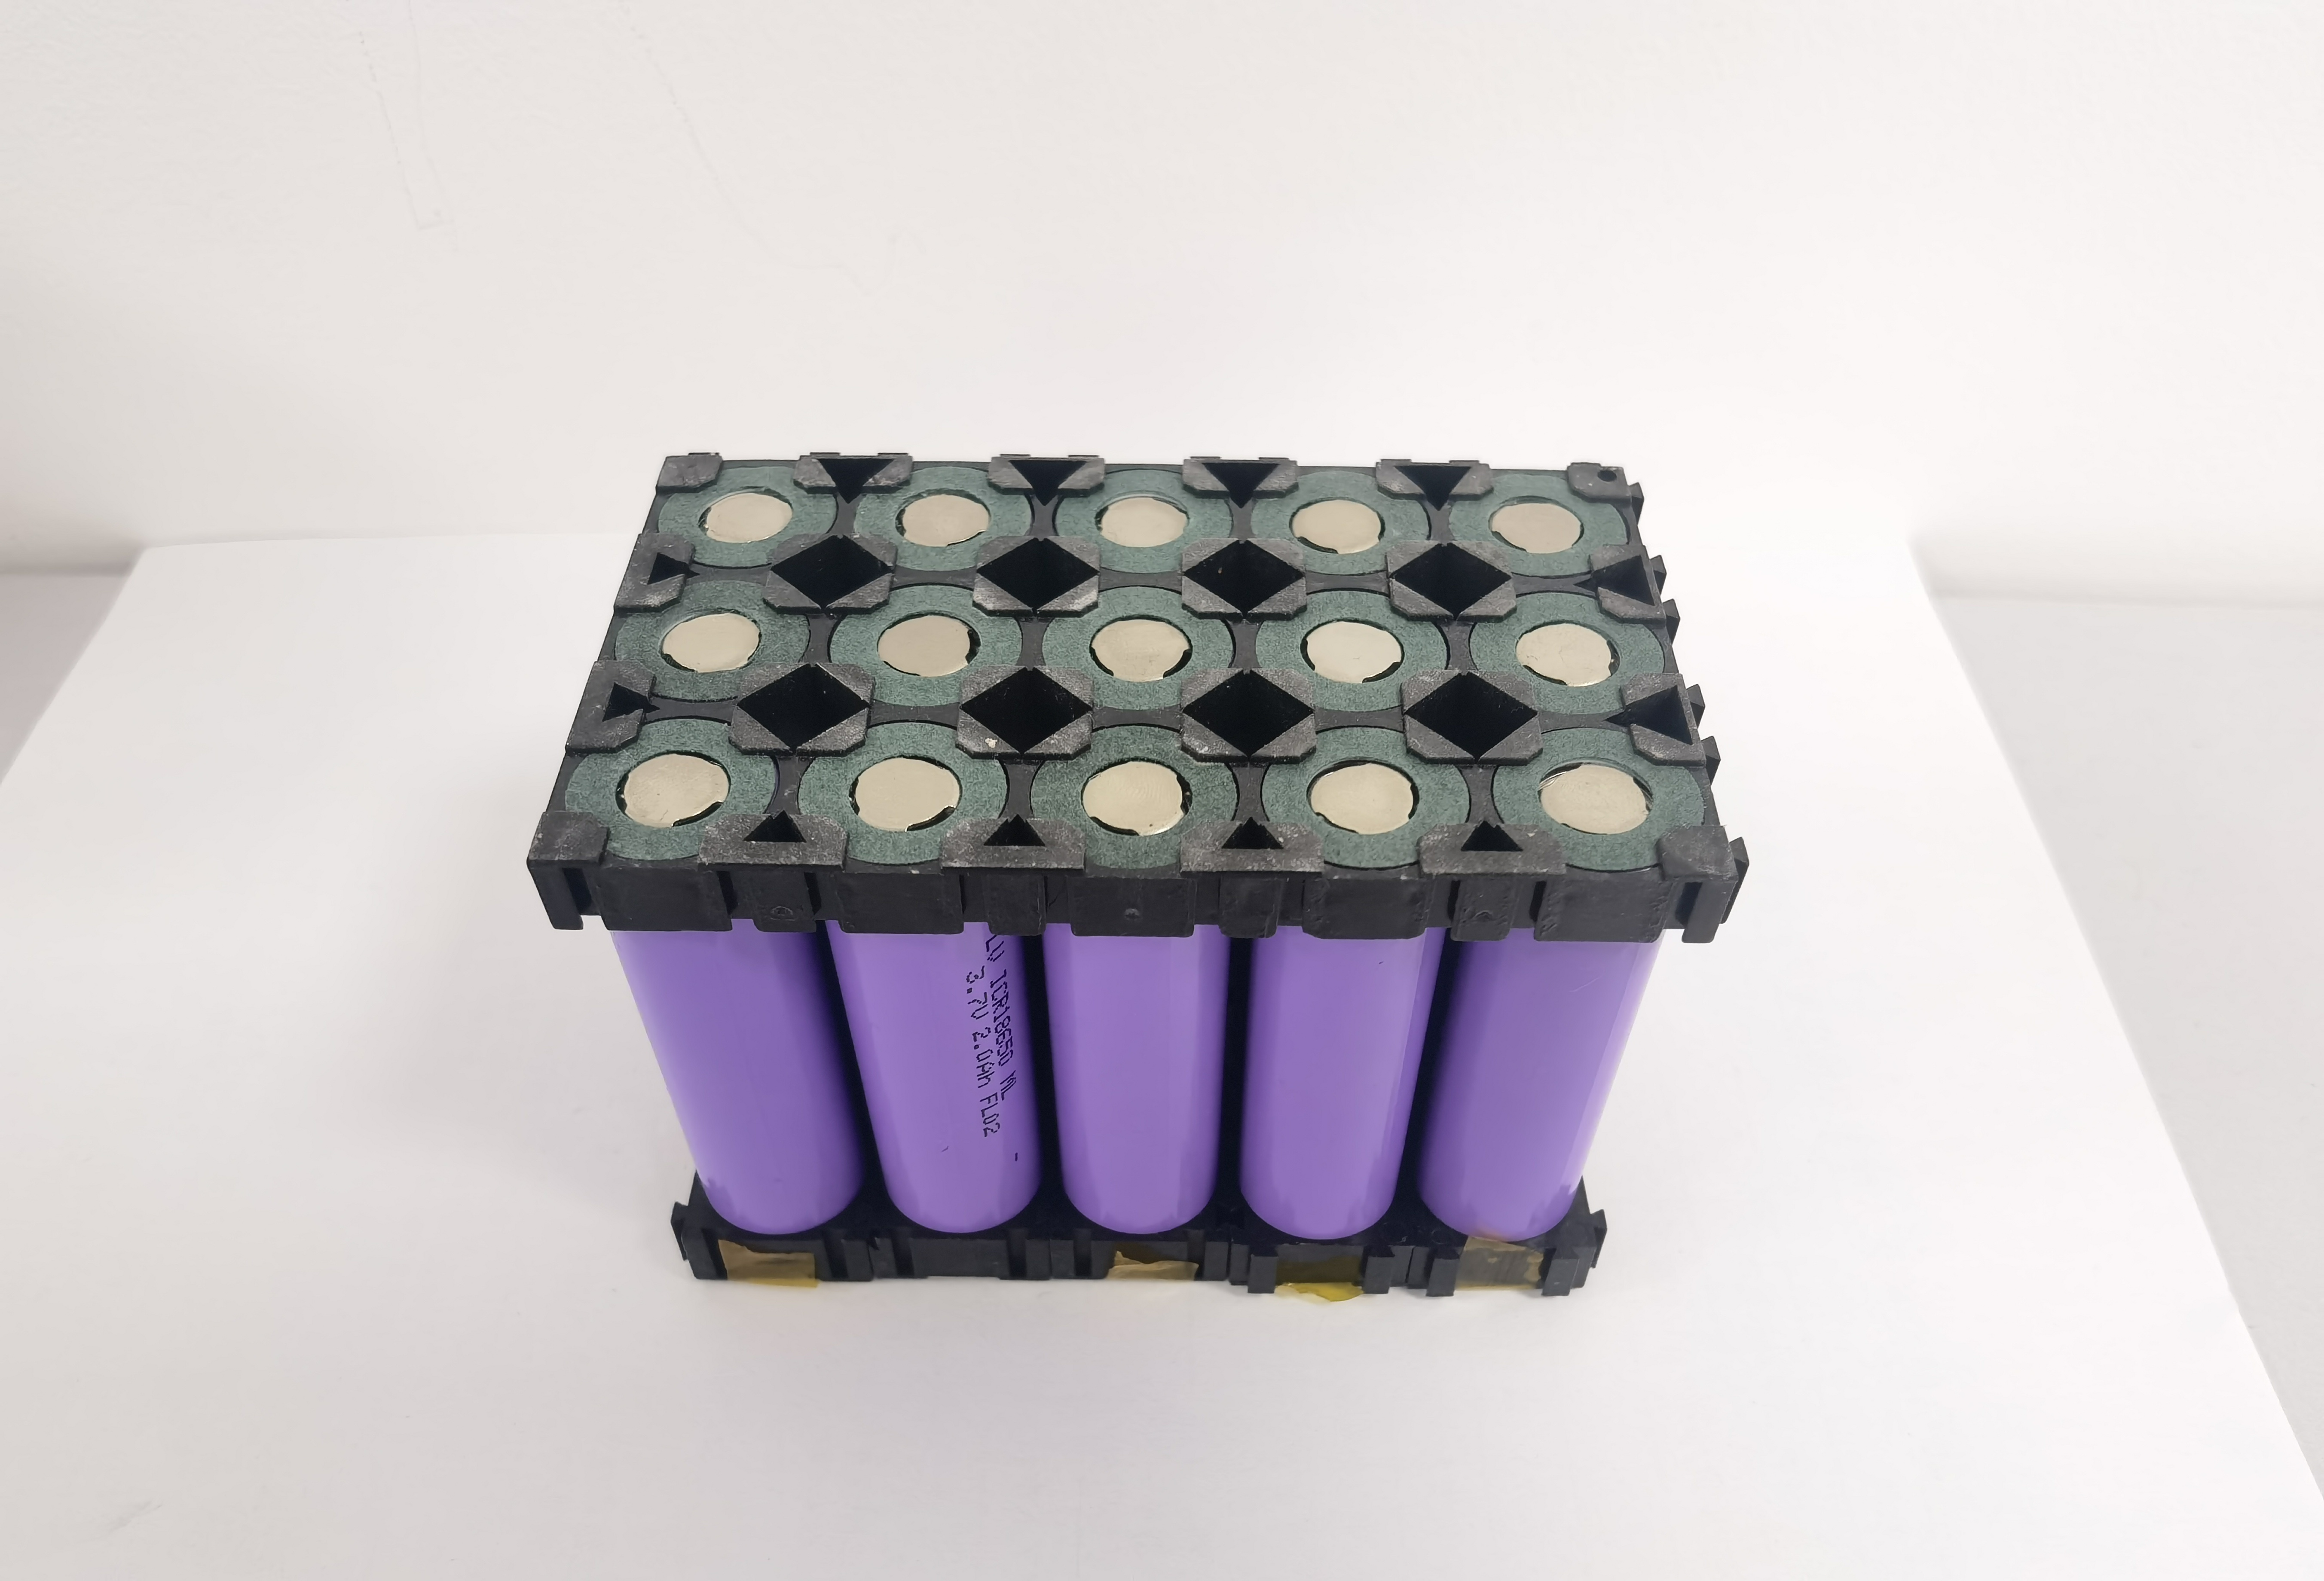
\includegraphics[width=\textwidth]{../attachments/IMG_20230411_225909.jpg}
\caption{The computational flowchart of the proposed method in this paper.}\label{fig:flowchart}
\end{figure}
\section{Case Study}

This section presents a case study to demonstrate the effectiveness of the proposed method.
A more intricate structure, which integrates the two previously proposed structures, is proposed.
The effectiveness of the aforementioned algorithm is substantiated on this structure to confirm its applicability in practical scenarios.
Moreover, the algorithm's versatility is also established through its application in complex cases such as the presence of isolated battery cell.

\subsection{Determination of a new RBS structure}

\begin{figure}[htbp]
    \centering
    \begin{subfigure}[b]{0.45\textwidth}
        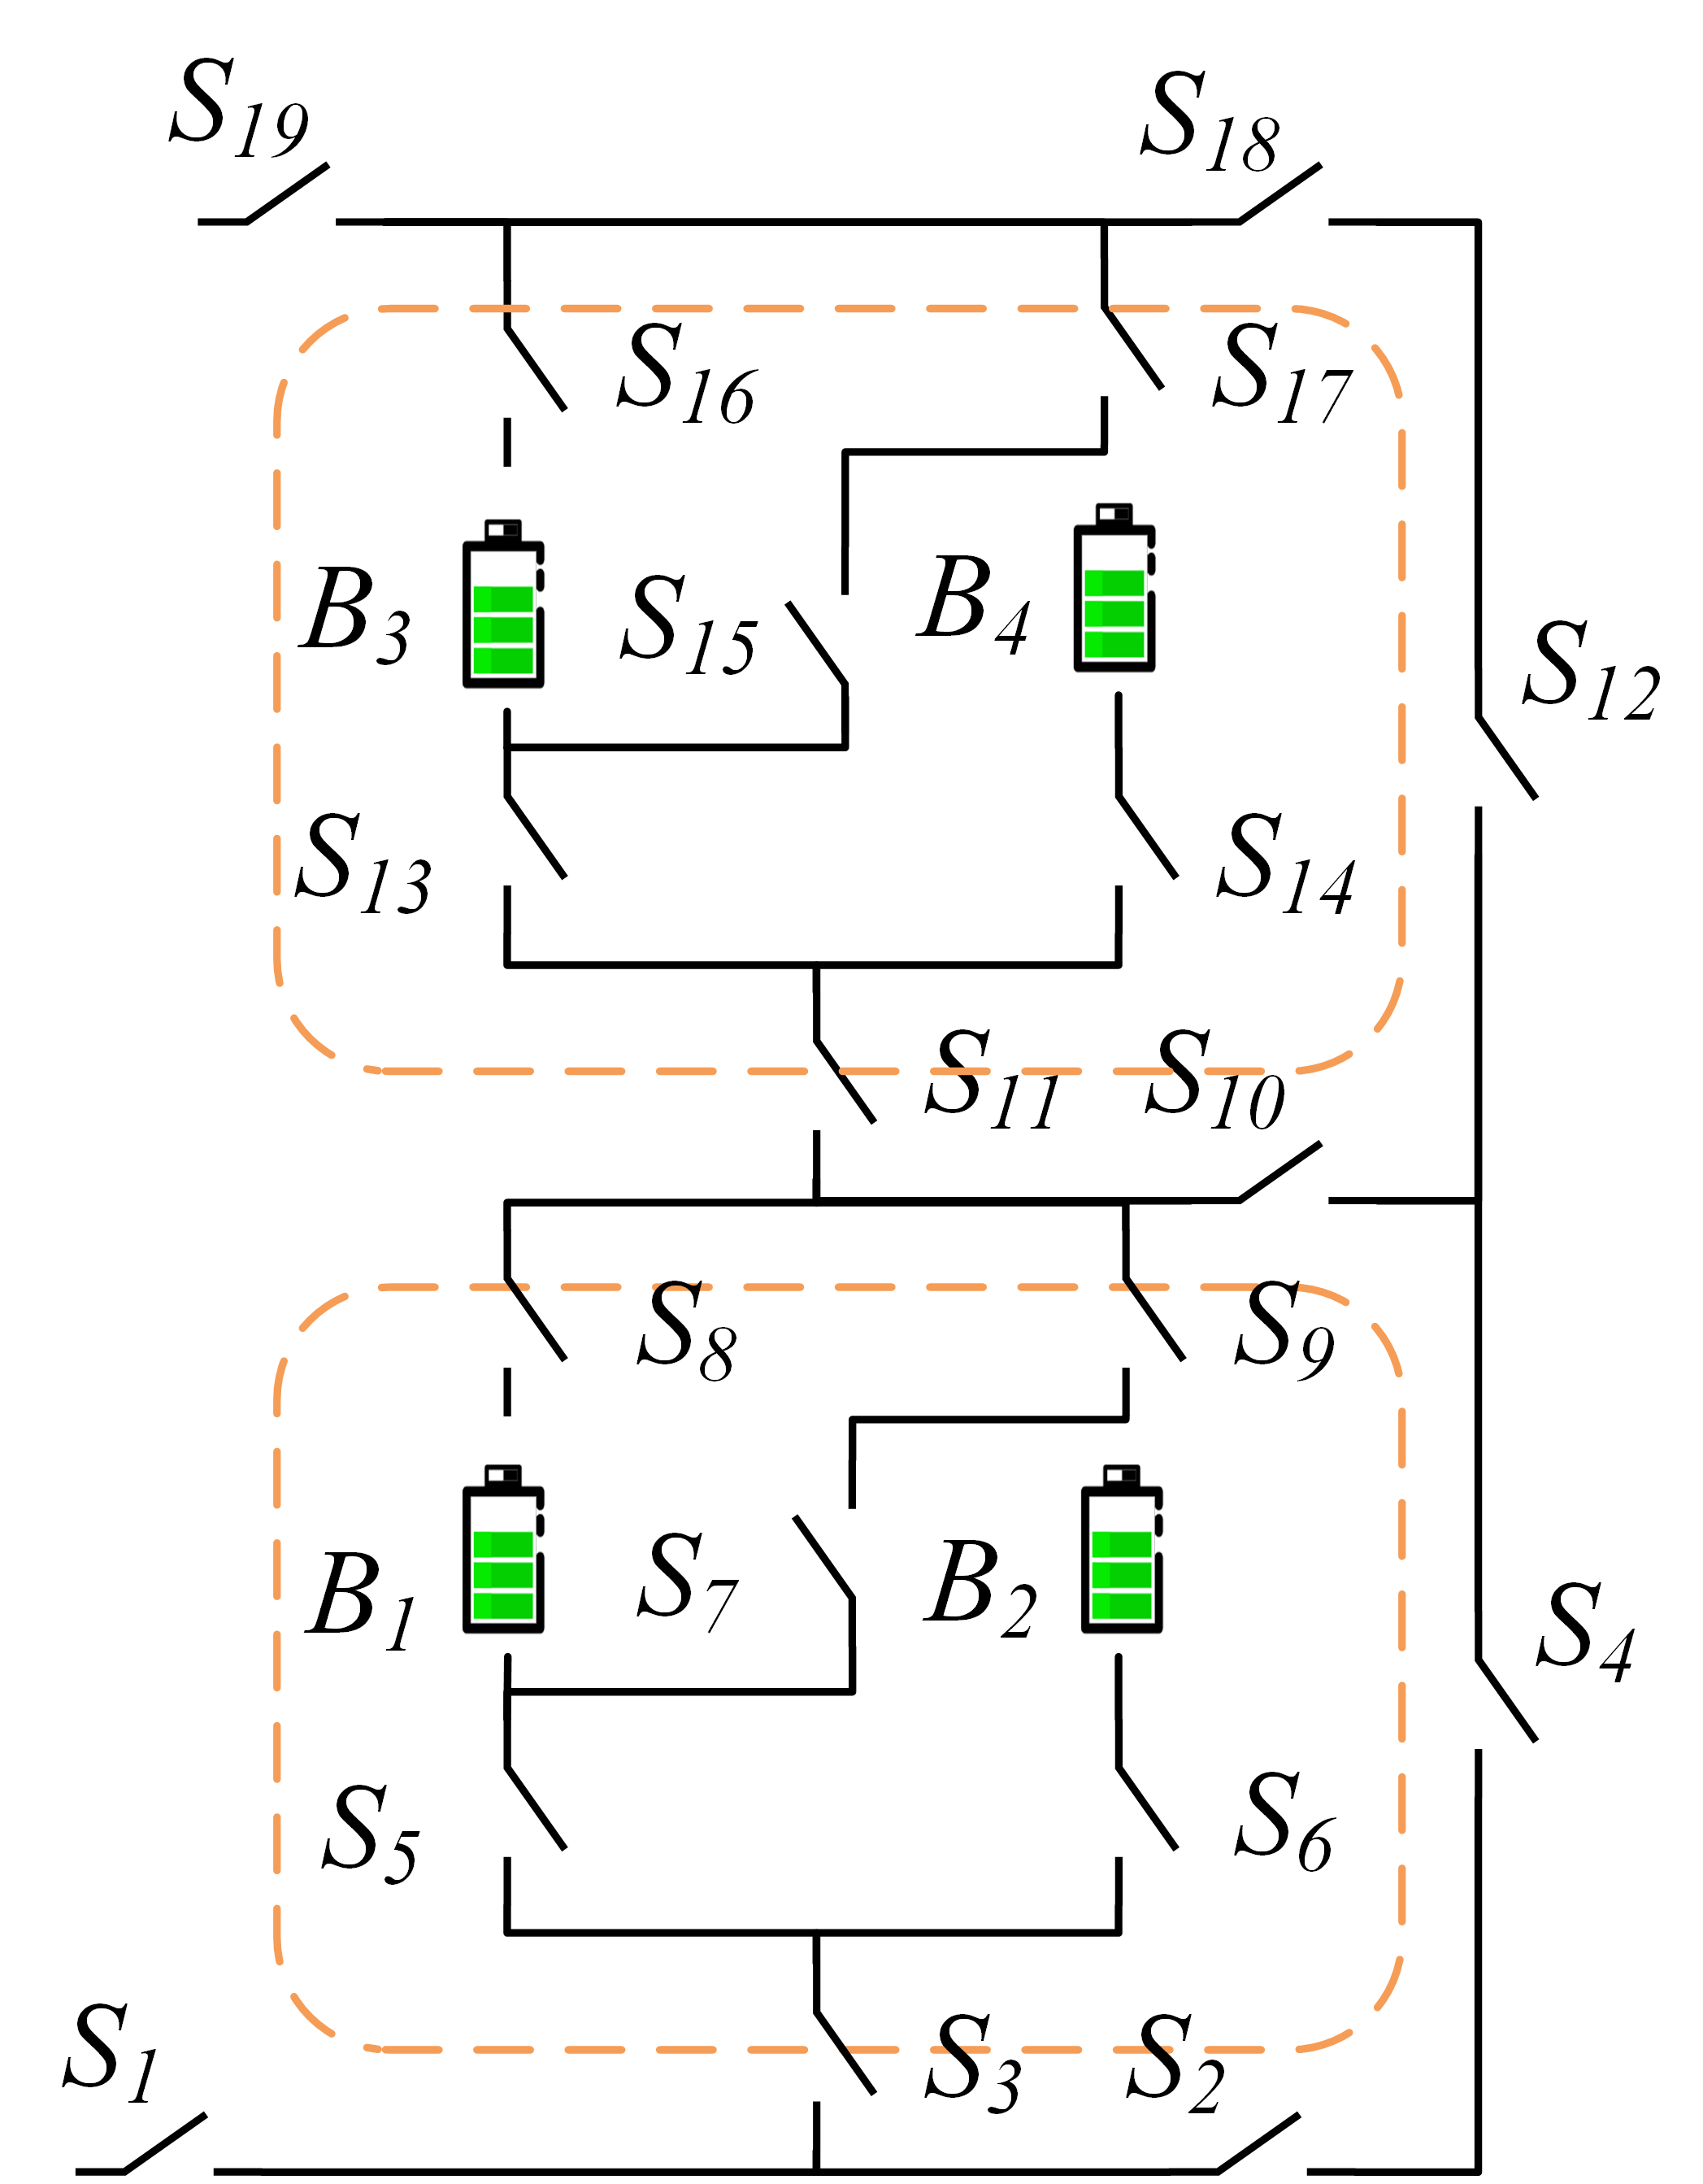
\includegraphics[width=\textwidth]{../attachments/arch-ef.png}
        \caption{}
        \label{fig:arch-ef}
    \end{subfigure}
    \hspace{0.05\textwidth}
    \begin{subfigure}[b]{0.45\textwidth}
        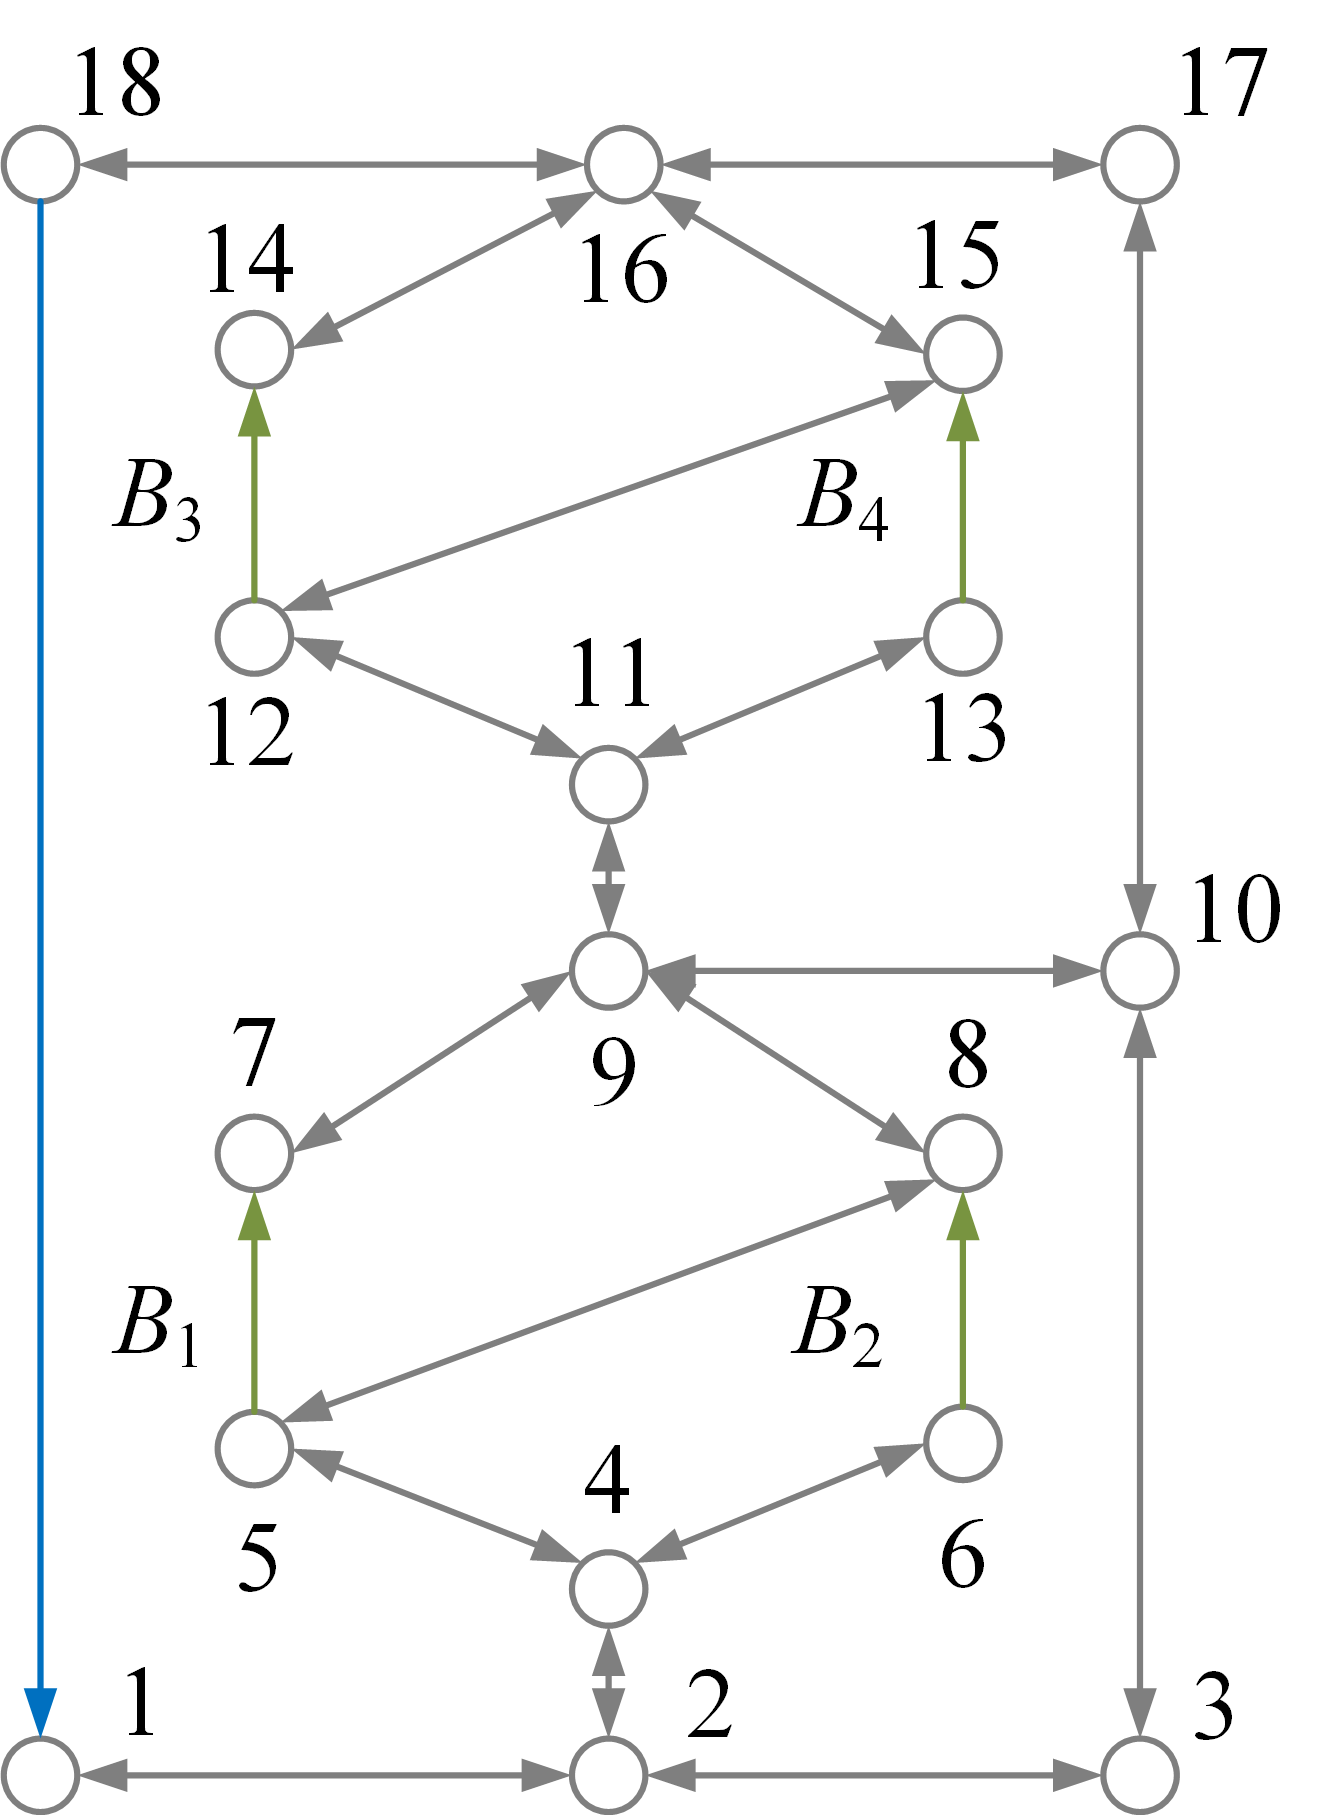
\includegraphics[width=\textwidth]{../attachments/ef-topo.png}
        \caption{}
        \label{fig:ef-topo}
    \end{subfigure}
    \caption{
        (a) The new RBS structure proposed in this paper, which is obtained by replacing the batteries in Fig. \ref{fig:arch-e} with the structure in Fig. \ref{fig:arch-f}, as shown in the dashed boxes in the figure.
        (b) The corresponding topologic model of the new RBS structure, which is a directed graph.
        The nodes represent the connection points of the battery cells and/or the switches.
        The green,gray and blue directed edges represent the battery cells, the switches and the external electrical appliance, respectively.
    }
\end{figure}

The RBS structure proposed by Lawson et al\cite{lawsonSoftwareConfigurableBattery2012}, shown in Fig. \ref{fig:arch-e}, easily enables the isolation of arbitrary cells or the addition of redundant cells to the system, but these cells are limited to being connected in series only and the switch between cells connection modes is not flexible. 
In contrast, the structure proposed by Visairo et al\cite{visairoReconfigurableBatteryPack2008}, shown in Fig. \ref{fig:arch-f}, allows the flexibility to switch the cells between series, parallel and mixed series-parallel modes, thus allowing dynamic voltage adjustment according to the external load and improving energy conversion efficiency, but is not as simple as the structure by Lawson et al in terms of isolating cells or adding redundancy.
In order to combine the advantages of both structures, a new structure is obtained by replacing the batteries in Fig. \ref{fig:arch-e} with the structure in Fig. \ref{fig:arch-f}, as shown in Fig. \ref{fig:arch-ef}.
This more complex structure has the structure of Lawson et al.\cite{lawsonSoftwareConfigurableBattery2012} as the main frame and the structure of Visairo et al.\cite{visairoReconfigurableBatteryPack2008} as the substructure.
In this way, the circuit topology of the substructure (i.e. the structure in the box in Fig. \ref{fig:arch-ef}) can be changed to enable dynamic and flexible voltage adjustment according to the load, while at the same time taking advantage of the ease of battery isolation and increased redundancy of the main frame.
The next subsections will use this structure with 4 battery cells and 19 switches as an example to demonstrate the effectiveness of the proposed algorithm.

\subsection{Calculation details and result}

The graph in Fig. \ref{fig:ef-topo} represents the topologic model based on the new RBS structure mentioned in the last subsection (Fig. \ref{fig:arch-ef}).
The model is presented in the form of a directed graph, capturing the connection relationship between the battery and switch in the circuit.
Battery cell 1, 2, 3, and 4 are represented by green directed edges in the graph, while nineteen switches are represented by gray directed edges with opposite directions.
The external electrical appliance is considered as a directed edge from the cathode of the RBS ( node $18$ in the graph) to the anode ( node $1$ in the graph), represented as the blue directed edge in the graph.
Totally, there are 19 nodes and 43 edges in the graph.


Based on the node-edge relationship given in Fig. \ref{fig:ef-topo}, the incidence matrix $\bm{A}$ can be obtained according to Eq. \ref{eq:A}:
\begin{equation}
    \bm{A} = 
    \begin{bmatrix}
        \bm{A}_b & \bm{A}_s & \bm{A}_o
    \end{bmatrix},
\end{equation}

\begin{equation}
    \bm{A}_b^\T = 
    \begin{bmatrix}
        0 & 0 & 0 & 0 & 1 & 0 &-1 & 0 & 0 & 0 & 0 & 0 & 0 & 0 & 0 & 0 & 0 \\
        0 & 0 & 0 & 0 & 0 & 1 & 0 &-1 & 0 & 0 & 0 & 0 & 0 & 0 & 0 & 0 & 0 \\
        0 & 0 & 0 & 0 & 0 & 0 & 0 & 0 & 0 & 0 & 0 & 1 & 0 &-1 & 0 & 0 & 0 \\
        0 & 0 & 0 & 0 & 0 & 0 & 0 & 0 & 0 & 0 & 0 & 0 & 1 & 0 &-1 & 0 & 0 \\
    \end{bmatrix},
\end{equation}

\begin{equation}
    \bm{A}_s^\T = 
    \begin{bmatrix}
        1 &-1 & 0 & 0 & 0 & 0 & 0 & 0 & 0 & 0 & 0 & 0 & 0 & 0 & 0 & 0 & 0 \\
        0 & 1 &-1 & 0 & 0 & 0 & 0 & 0 & 0 & 0 & 0 & 0 & 0 & 0 & 0 & 0 & 0 \\
        0 & 1 & 0 &-1 & 0 & 0 & 0 & 0 & 0 & 0 & 0 & 0 & 0 & 0 & 0 & 0 & 0 \\
        0 & 0 & 1 & 0 & 0 & 0 & 0 & 0 & 0 &-1 & 0 & 0 & 0 & 0 & 0 & 0 & 0 \\
        0 & 0 & 0 & 1 &-1 & 0 & 0 & 0 & 0 & 0 & 0 & 0 & 0 & 0 & 0 & 0 & 0 \\
        0 & 0 & 0 & 1 & 0 &-1 & 0 & 0 & 0 & 0 & 0 & 0 & 0 & 0 & 0 & 0 & 0 \\
        0 & 0 & 0 & 0 & 1 & 0 & 0 &-1 & 0 & 0 & 0 & 0 & 0 & 0 & 0 & 0 & 0 \\
        0 & 0 & 0 & 0 & 0 & 0 & 1 & 0 &-1 & 0 & 0 & 0 & 0 & 0 & 0 & 0 & 0 \\
        0 & 0 & 0 & 0 & 0 & 0 & 0 & 1 &-1 & 0 & 0 & 0 & 0 & 0 & 0 & 0 & 0 \\
        0 & 0 & 0 & 0 & 0 & 0 & 0 & 0 & 1 &-1 & 0 & 0 & 0 & 0 & 0 & 0 & 0 \\
        0 & 0 & 0 & 0 & 0 & 0 & 0 & 0 & 1 & 0 &-1 & 0 & 0 & 0 & 0 & 0 & 0 \\
        0 & 0 & 0 & 0 & 0 & 0 & 0 & 0 & 0 & 1 & 0 & 0 & 0 & 0 & 0 & 0 &-1 \\
        0 & 0 & 0 & 0 & 0 & 0 & 0 & 0 & 0 & 0 & 1 &-1 & 0 & 0 & 0 & 0 & 0 \\
        0 & 0 & 0 & 0 & 0 & 0 & 0 & 0 & 0 & 0 & 1 & 0 &-1 & 0 & 0 & 0 & 0 \\
        0 & 0 & 0 & 0 & 0 & 0 & 0 & 0 & 0 & 0 & 0 & 1 & 0 & 0 &-1 & 0 & 0 \\
        0 & 0 & 0 & 0 & 0 & 0 & 0 & 0 & 0 & 0 & 0 & 0 & 0 & 1 & 0 &-1 & 0 \\
        0 & 0 & 0 & 0 & 0 & 0 & 0 & 0 & 0 & 0 & 0 & 0 & 0 & 0 & 1 &-1 & 0 \\
        0 & 0 & 0 & 0 & 0 & 0 & 0 & 0 & 0 & 0 & 0 & 0 & 0 & 0 & 0 & 1 &-1 \\
        0 & 0 & 0 & 0 & 0 & 0 & 0 & 0 & 0 & 0 & 0 & 0 & 0 & 0 & 0 & 1 & 0 \\
    \end{bmatrix},
\end{equation}

\begin{equation}
    \bm{A}_o^\T = 
    \begin{bmatrix}
       -1 & 0 & 0 & 0 & 0 & 0 & 0 & 0 & 0 & 0 & 0 & 0 & 0 & 0 & 0 & 0 & 0 \\
    \end{bmatrix}.
\end{equation}
The state matrix $\bm{X}$ is determined by the switches' state, that is, the specific configuration of the RBS.
For example, when switch $S_1$, $S_3$, $S_5$, $S_6$, $S_8$, $S_9$, $S_{11}$, $S_{13}$, $S_{14}$, $S_{16}$, $S_{17}$ and $S_{19}$ are ON, and the rest of the switches are OFF, the state matrix $\bm{X}$ is given by
\begin{equation}
    \bm{X} = diag(
    \underbrace{1,0,1,0,1,1,0,1,1,0,1,0,1,1,0,1,1,0,1}_{\text{switches}},
    \underbrace{1,1,1,1}_{\text{batteries}},
    1
    ).
\end{equation}
By substituting the above specific values of $\bm{A}$ and $\bm{X}$ above into Eqs. \ref{eq:Yn}, \ref{eq:I_o}, \ref{eq:I_b} and \ref{eq:eta} in turn, the $\eta$ at the current situation, i.e. battery cell $B_1$ and $B_2$, $B_3$ and $B_4$ are connected in parallel with each other, and then connected in series to supply the external electrical appliance, can be obtained after the sequential calculation.
The results are shown in Tab. \ref{tab:given_x}.

\begin{table}[htbp]
  \centering
    \caption{Calculating result of the output current $I_o$, battery current $\bm{I}_b$ and ratio $\eta$ for a specificed switches state $\bm{X}_m$ in the structure combining Lawson et al.\cite{lawsonSoftwareConfigurableBattery2012} and Visairo et al.\cite{visairoReconfigurableBatteryPack2008} with 4 battery cells and 19 switches.}
    \begin{tabular}{cc}
    \toprule
        Structure & 4 battery cells and 19 switches  \\
        % Structure & combining Lawson et al.\cite{lawsonSoftwareConfigurableBattery2012} and Visairo et al.\cite{visairoReconfigurableBatteryPack2008} with 4 battery cells and 19 switches  \\
    \midrule
    Switch ON & 1,3,5,6,8,9,11,13,14,16,17,19 \\
        $\bm{X}_s$ & $\diag(1,0,1,0,1,1,0,1,1,0,1,0,1,1,0,1,1,0,1)$ \\
    \midrule
        $I_o$ & $2u_b/(R_o+r_b)$ \\
        $\bm{I}_b$ & $[u_b/(R_o+r_b),u_b/(R_o+r_b),u_b/(R_o+r_b),u_b/(R_o+r_b)]$ \\
        $\eta$     & 2 \\
    \bottomrule
    \end{tabular}%
  \label{tab:given_x}%
\end{table}%

The above gives the procedure for calculating the current and $\eta$ when the specified switches are given ON or OFF.
However, in order to calculate the MAC of the structure, i.e. the maximum $\eta$, it is necessary to find the corresponding switch state using a greedy strategy, as mentioned in subsection \ref{subsec:greedy_solution}.

Firstly, the weight $N_s$ in Eq. \ref{eq:weight} represents the total number of switches in the system, which is 19. 
By using this formula and the Dijkstra search strategy, the $SP$s of each cell can be obtained, as shown in Figs. \ref{fig:sp1} to \ref{fig:sp4}.
According to the greedy strategy, as many $SP$s as possible should be selected to get the MAC. 
In the first iteration, the $SP$s of all four batteries are selected, and the switch states on the paths are set to ON. 
The corresponding $\bm{X}_s$ are calculated using the previous method, and the currents of the batteries are obtained as $u_b/r_b$, $u_b/r_b$, $u_b/r_b$, and $u_b/r_b$. 
Since all batteries are short-circuited and the current of the battery exceeds the maximum allowed current $I_m$, this solution does not satisfy constraint \ref{eq:Ib_leq_Im} and is discarded. 
The second iteration is carried out using the dichotomy method, and two batteries are selected for the combination. 
Assuming that the selected combinations are $(B1, B2)$, the $\bm{X}_s$ obtained according to the $SP$s are substituted into the previous calculation, and the current of each battery is $u_b/r_b$, $u_b/r_b$, $0$, and $0$. 
This solution meets the condition. 
After that, the case of selecting three cells is considered. 
By similar calculations, it is determined that all solutions do not satisfy the constraint when three cells are selected. 
Finally, the MAC of this structure is $\eta=2$, and the related result is shown in Fig. \ref{fig:ef-mac} and Tab. \ref{tab:find_mac}.

\begin{figure}[htbp]
    \centering
    \begin{subfigure}[b]{0.45\textwidth}
        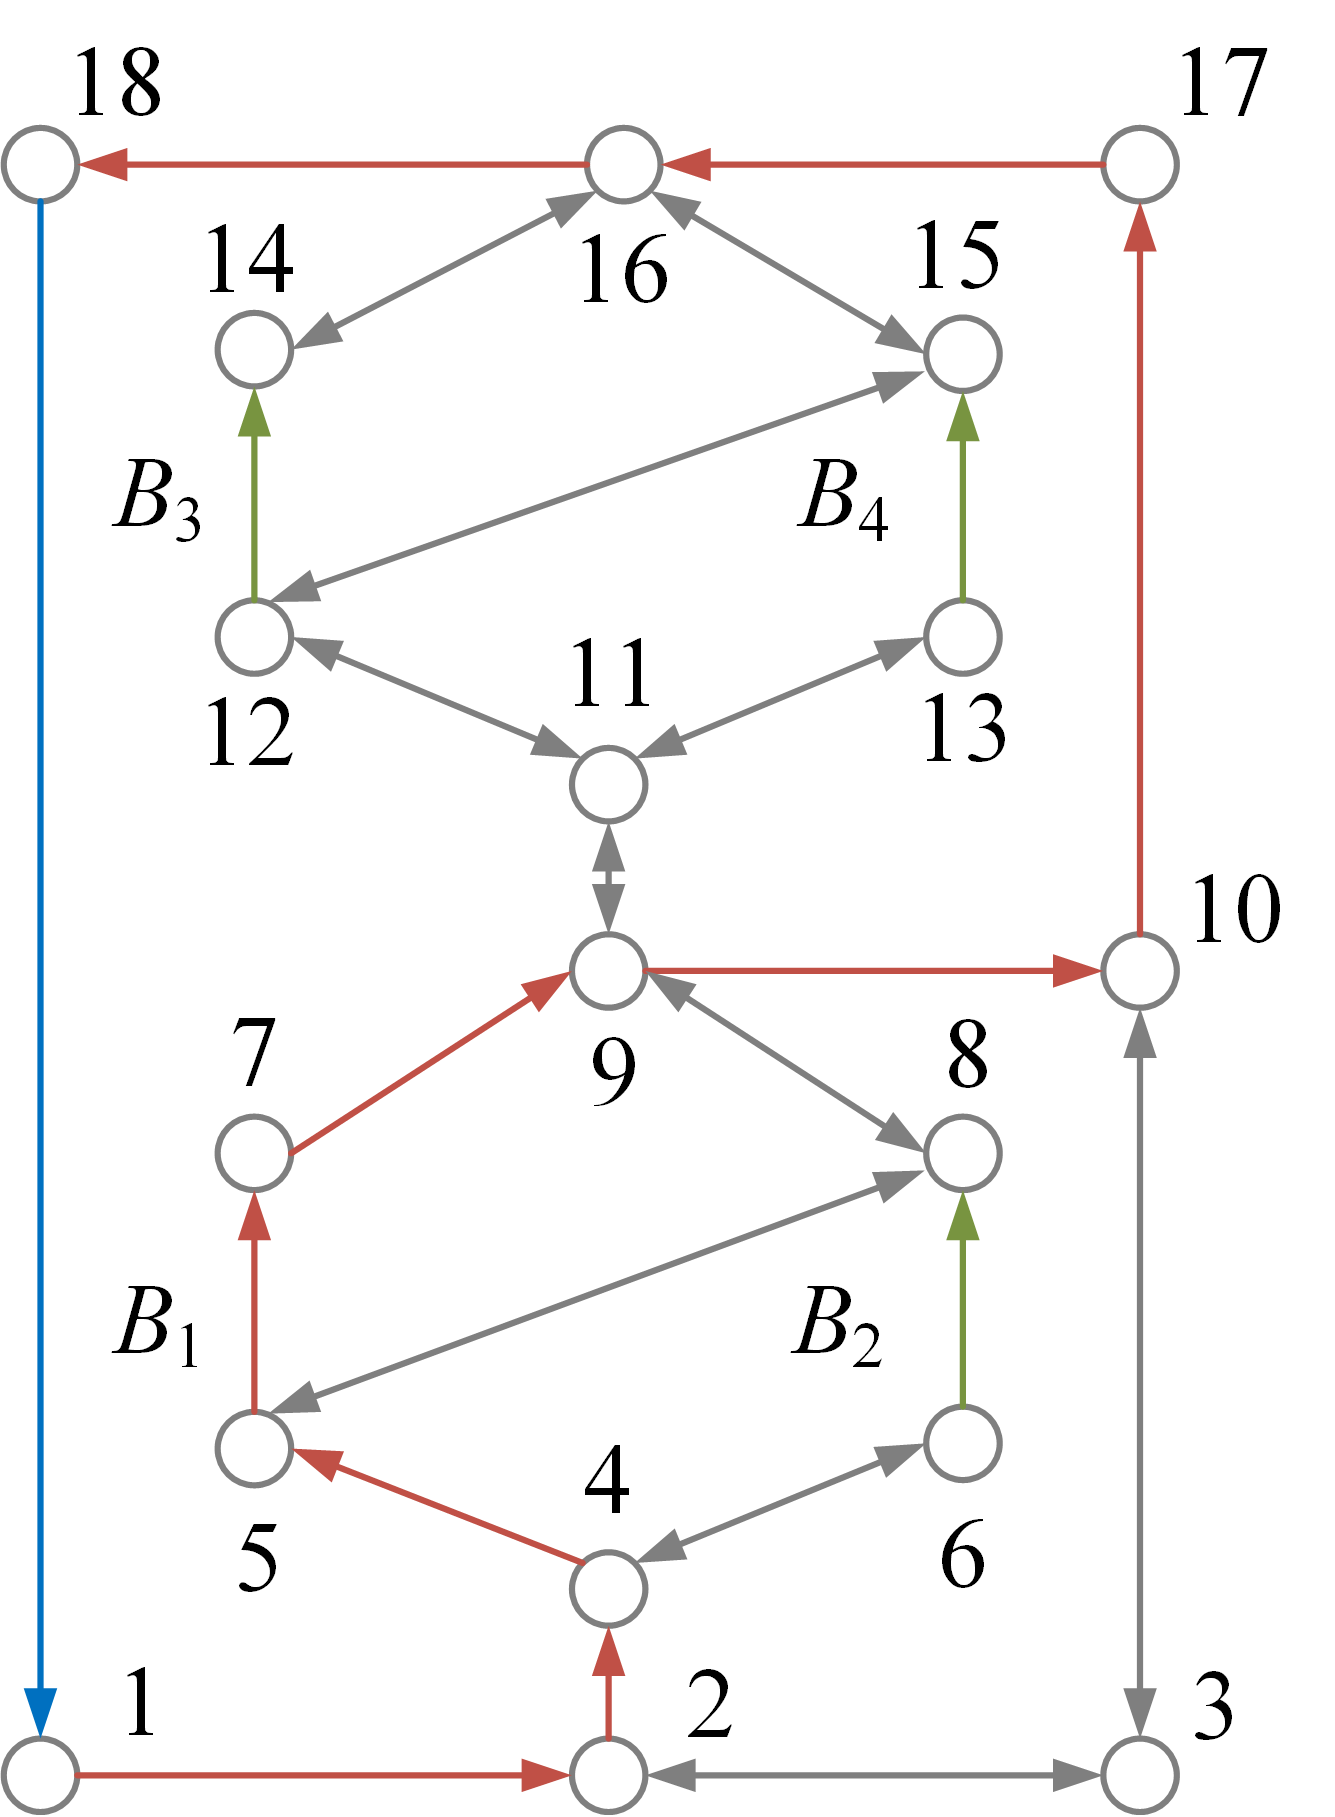
\includegraphics[width=\textwidth]{../attachments/ef-sp1.png}
        \caption{}
        \label{fig:sp1}
    \end{subfigure}
    \hspace{0.05\textwidth}
    \begin{subfigure}[b]{0.45\textwidth}
        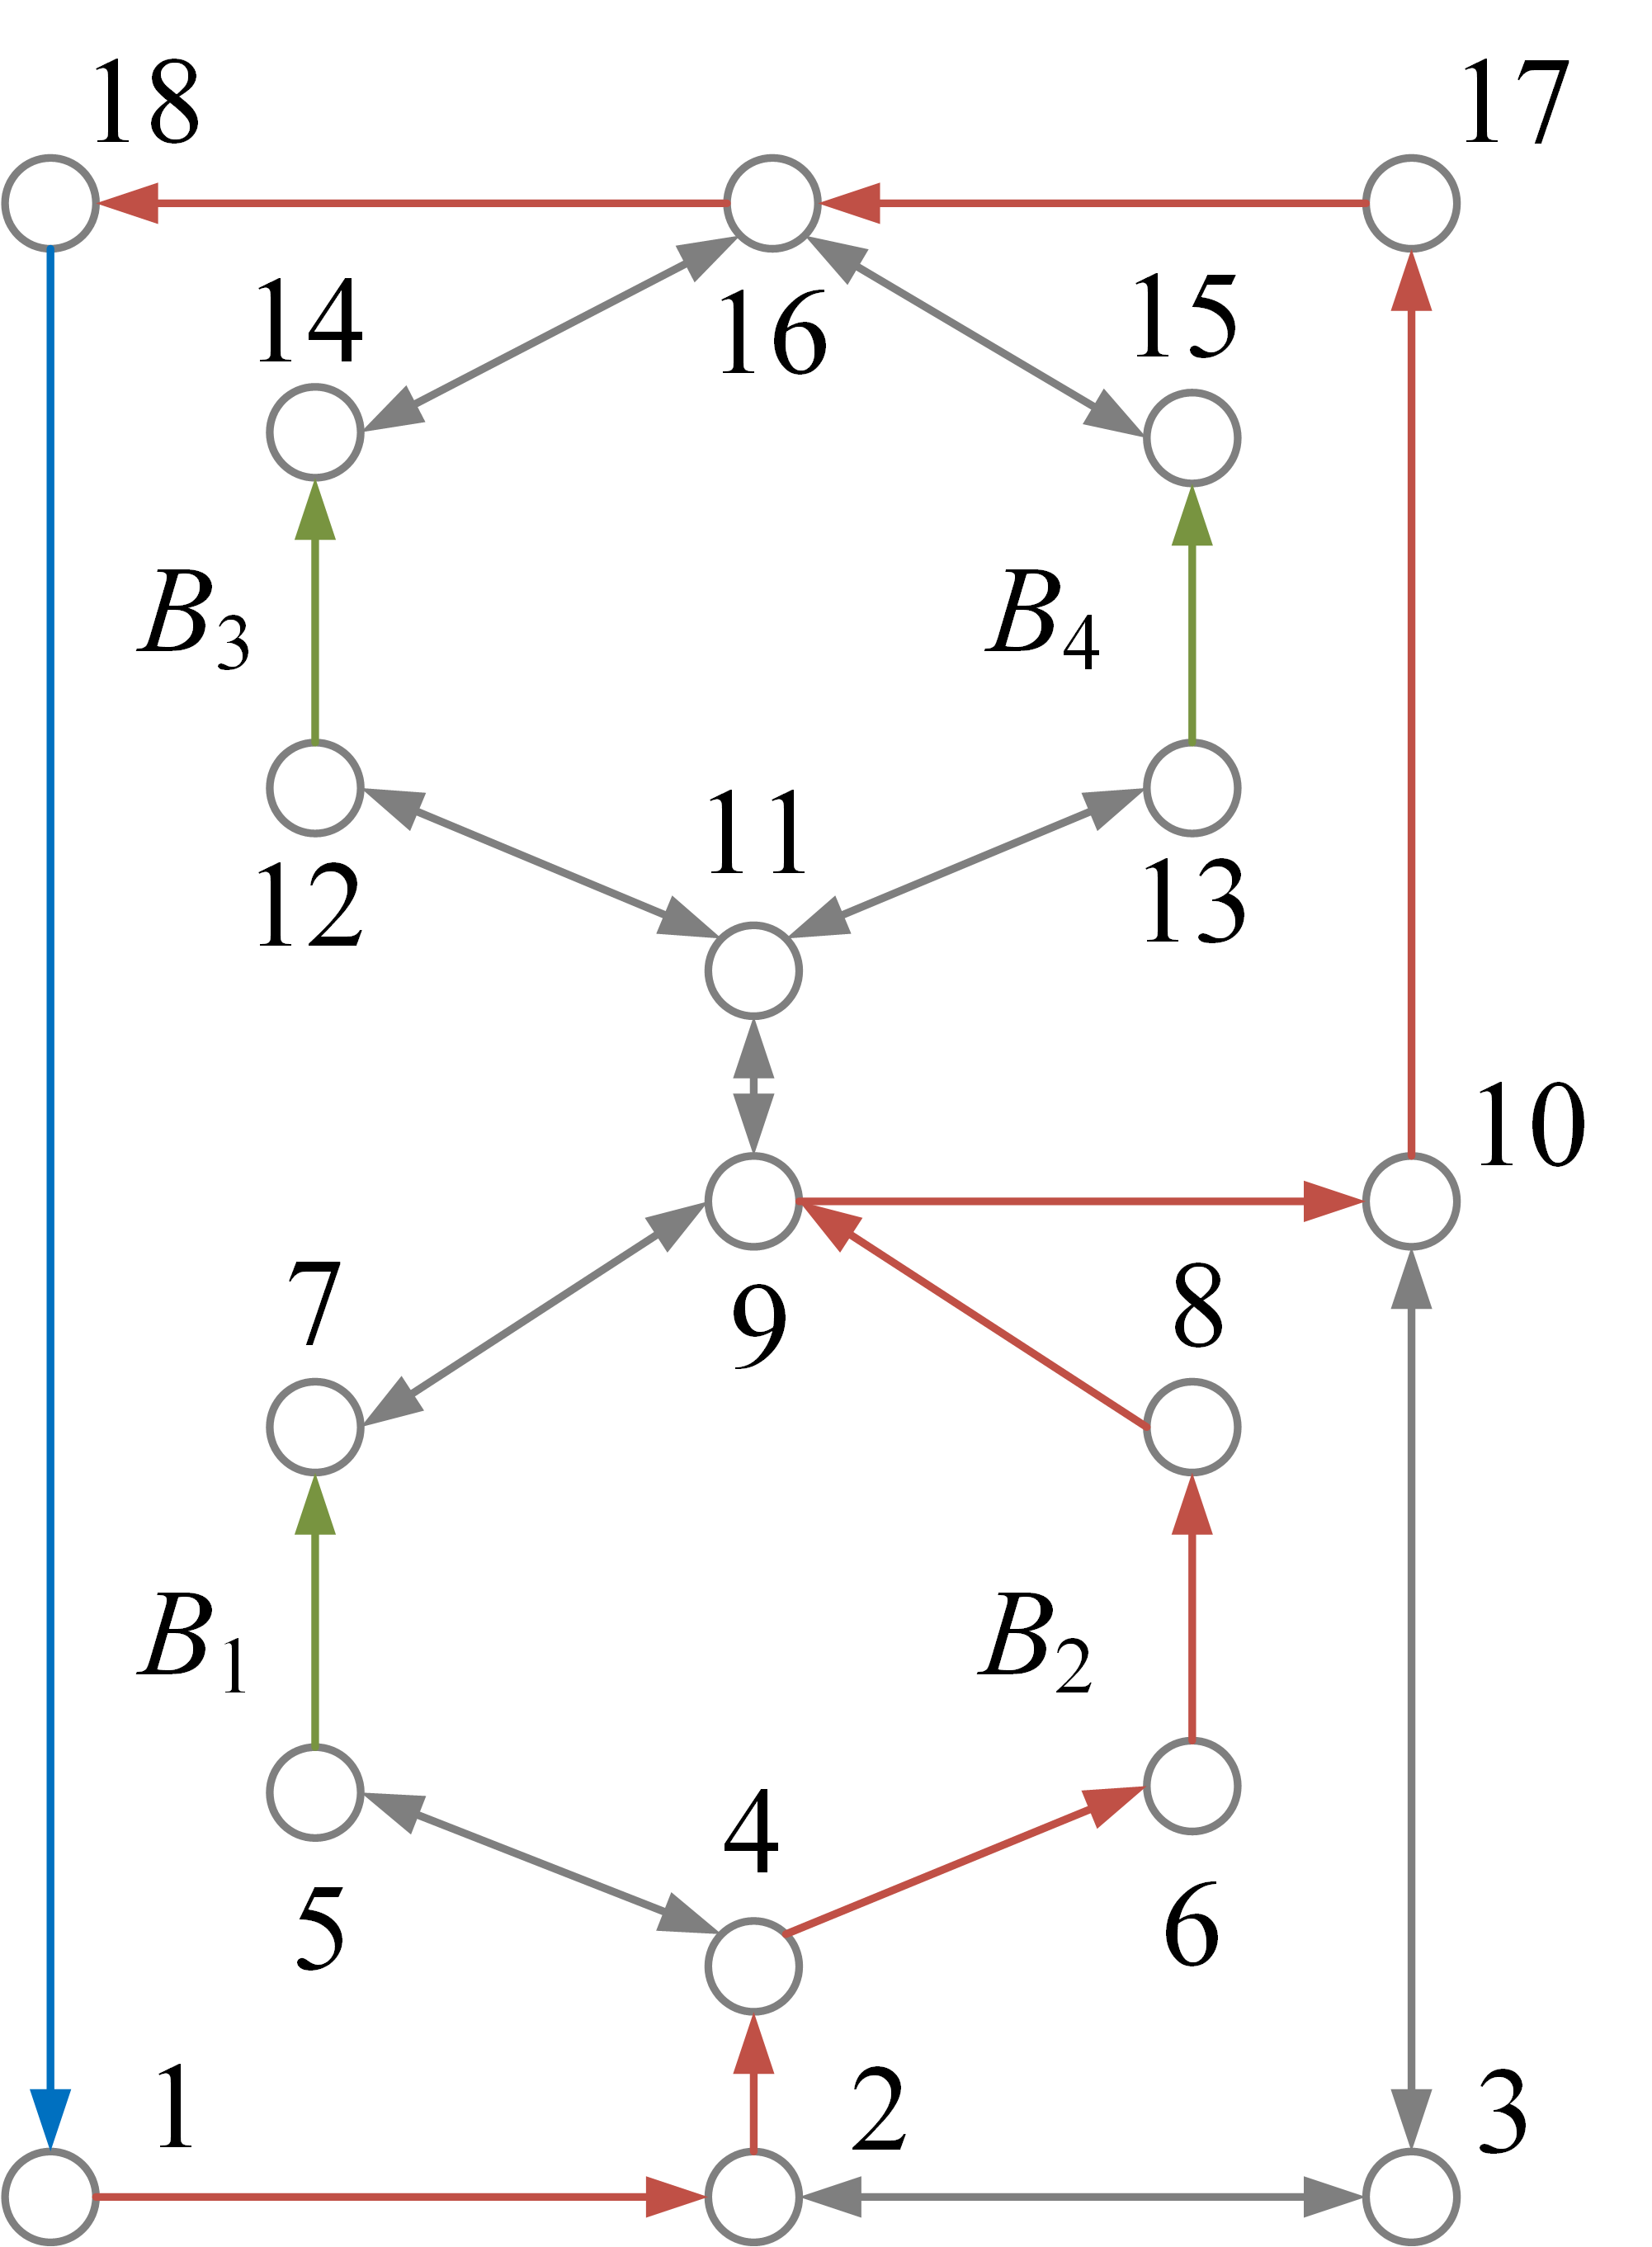
\includegraphics[width=\textwidth]{../attachments/ef-sp2.png}
        \caption{}
        \label{fig:sp2}
    \end{subfigure}
    \\
    \begin{subfigure}[b]{0.45\textwidth}
        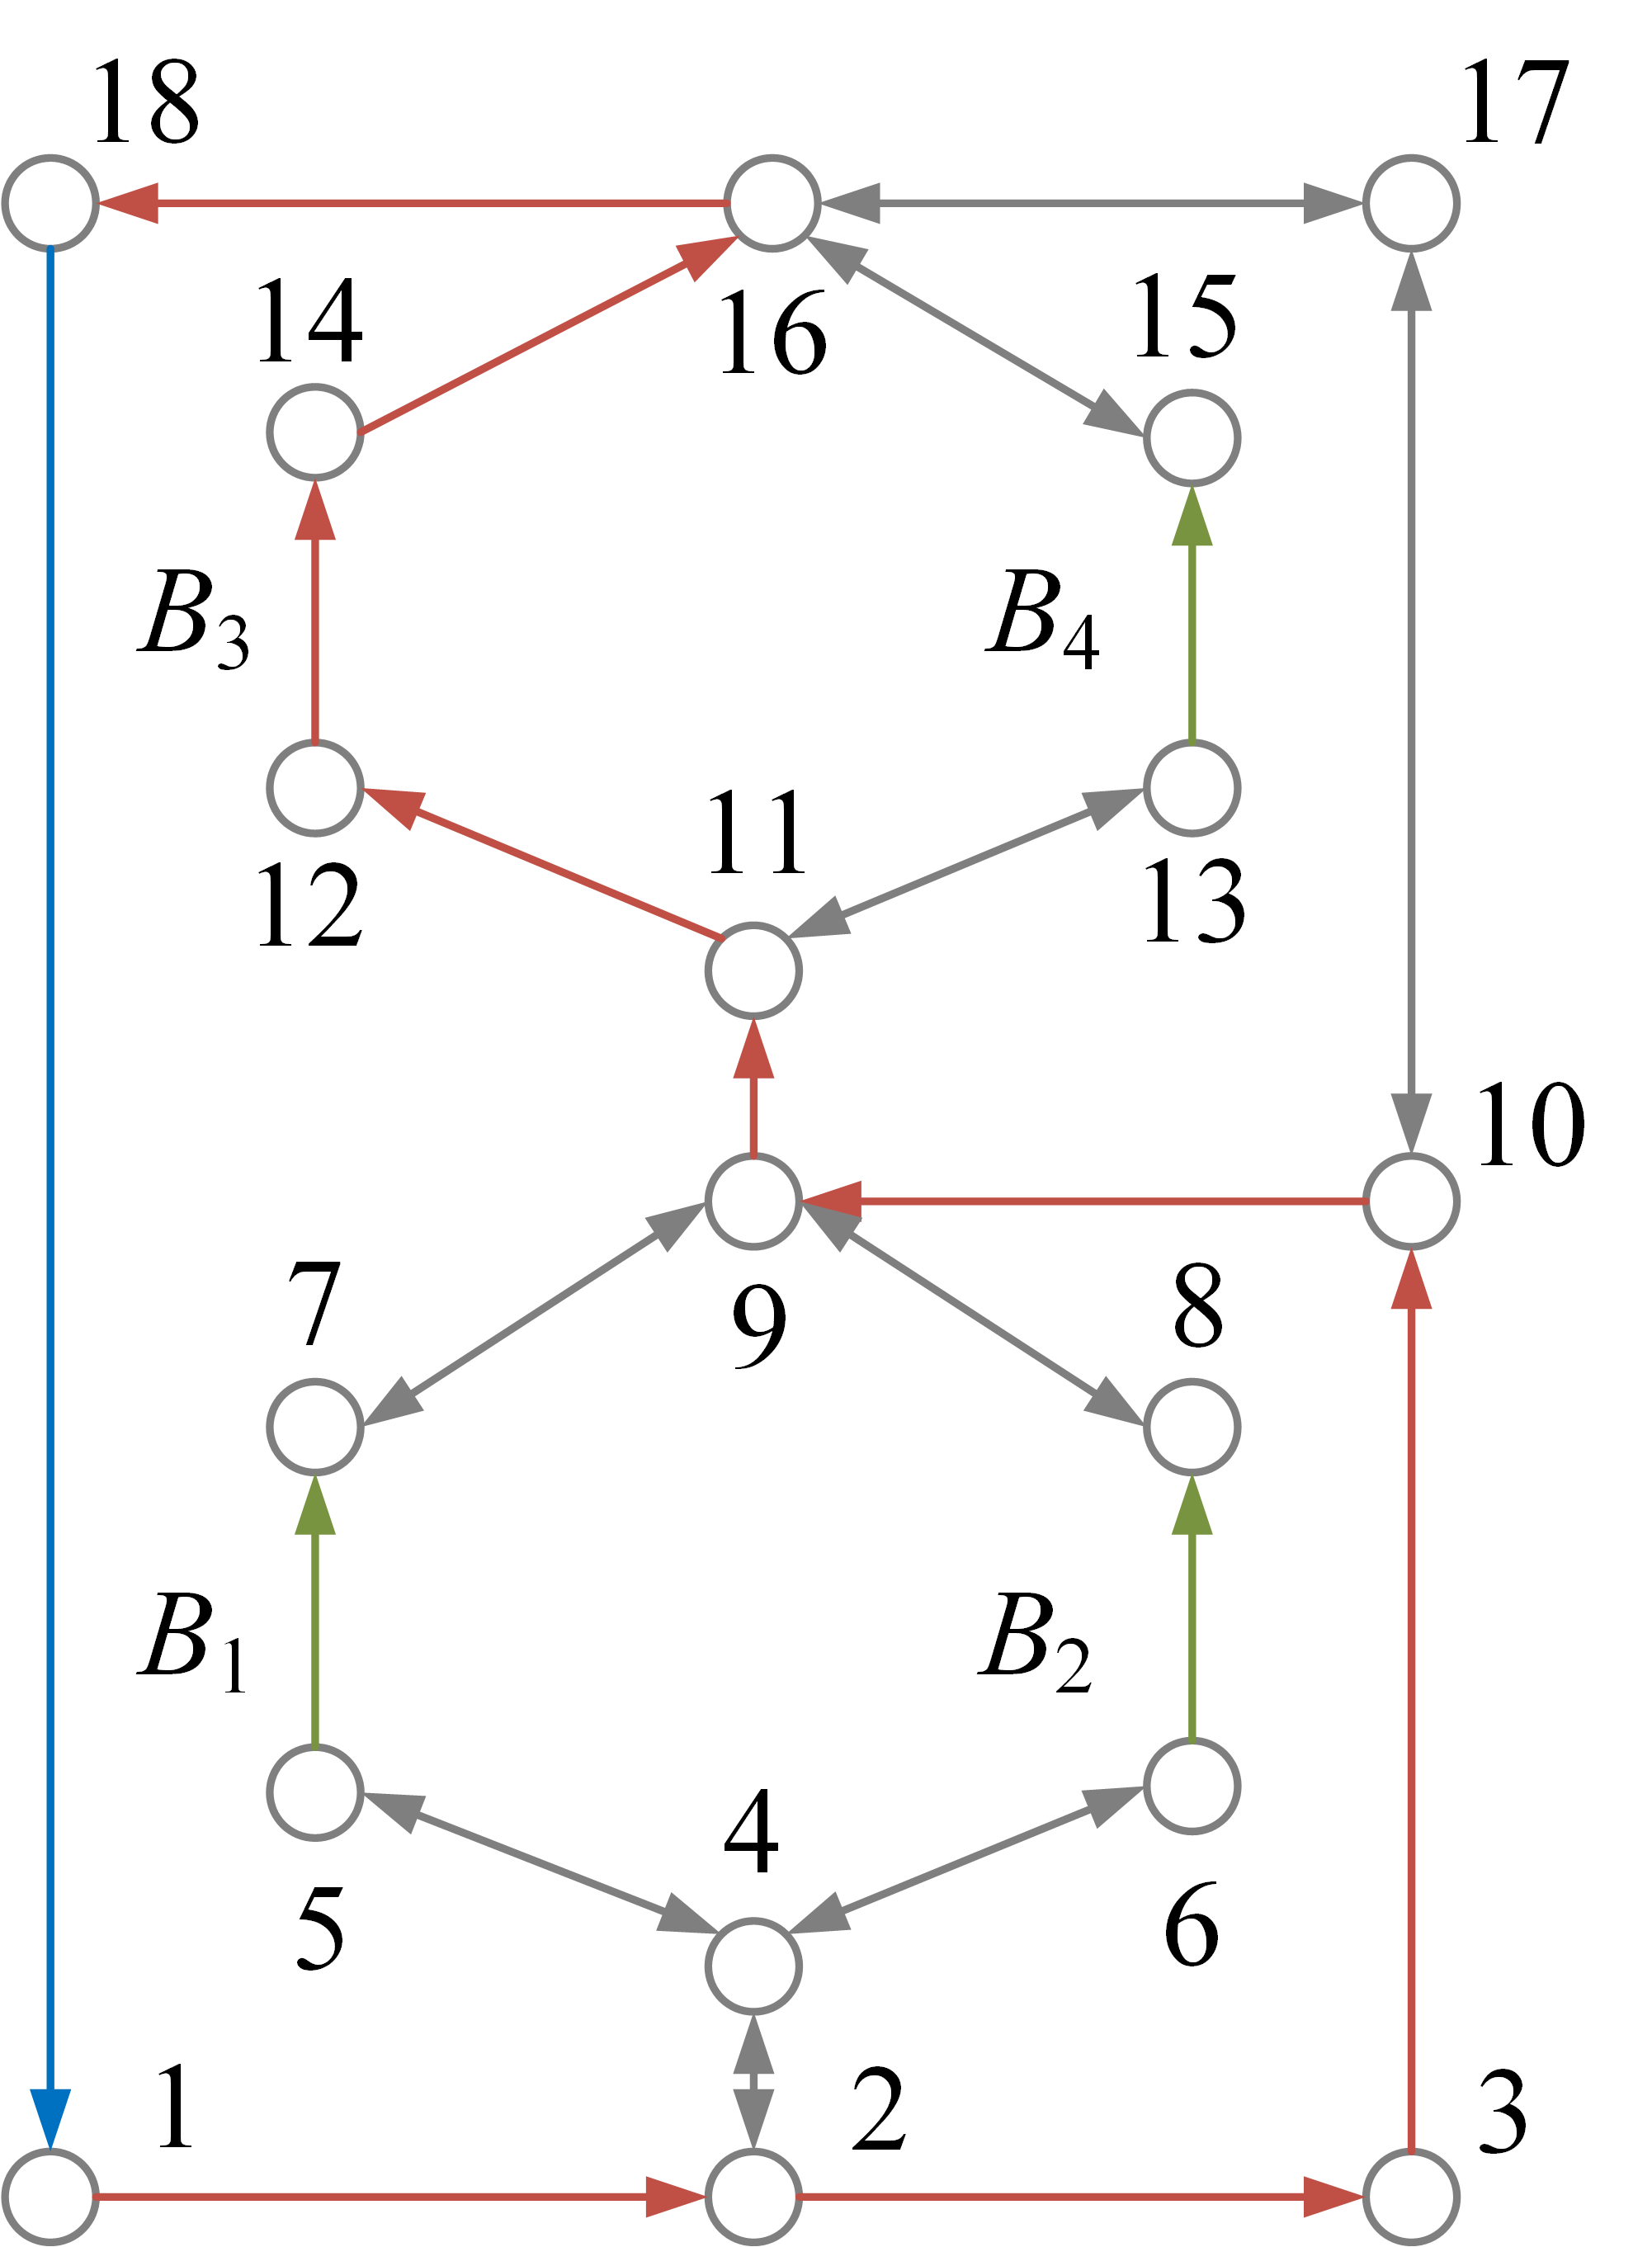
\includegraphics[width=\textwidth]{../attachments/ef-sp3.png}
        \caption{}
        \label{fig:sp3}
    \end{subfigure}
    \hspace{0.05\textwidth}
    \begin{subfigure}[b]{0.45\textwidth}
        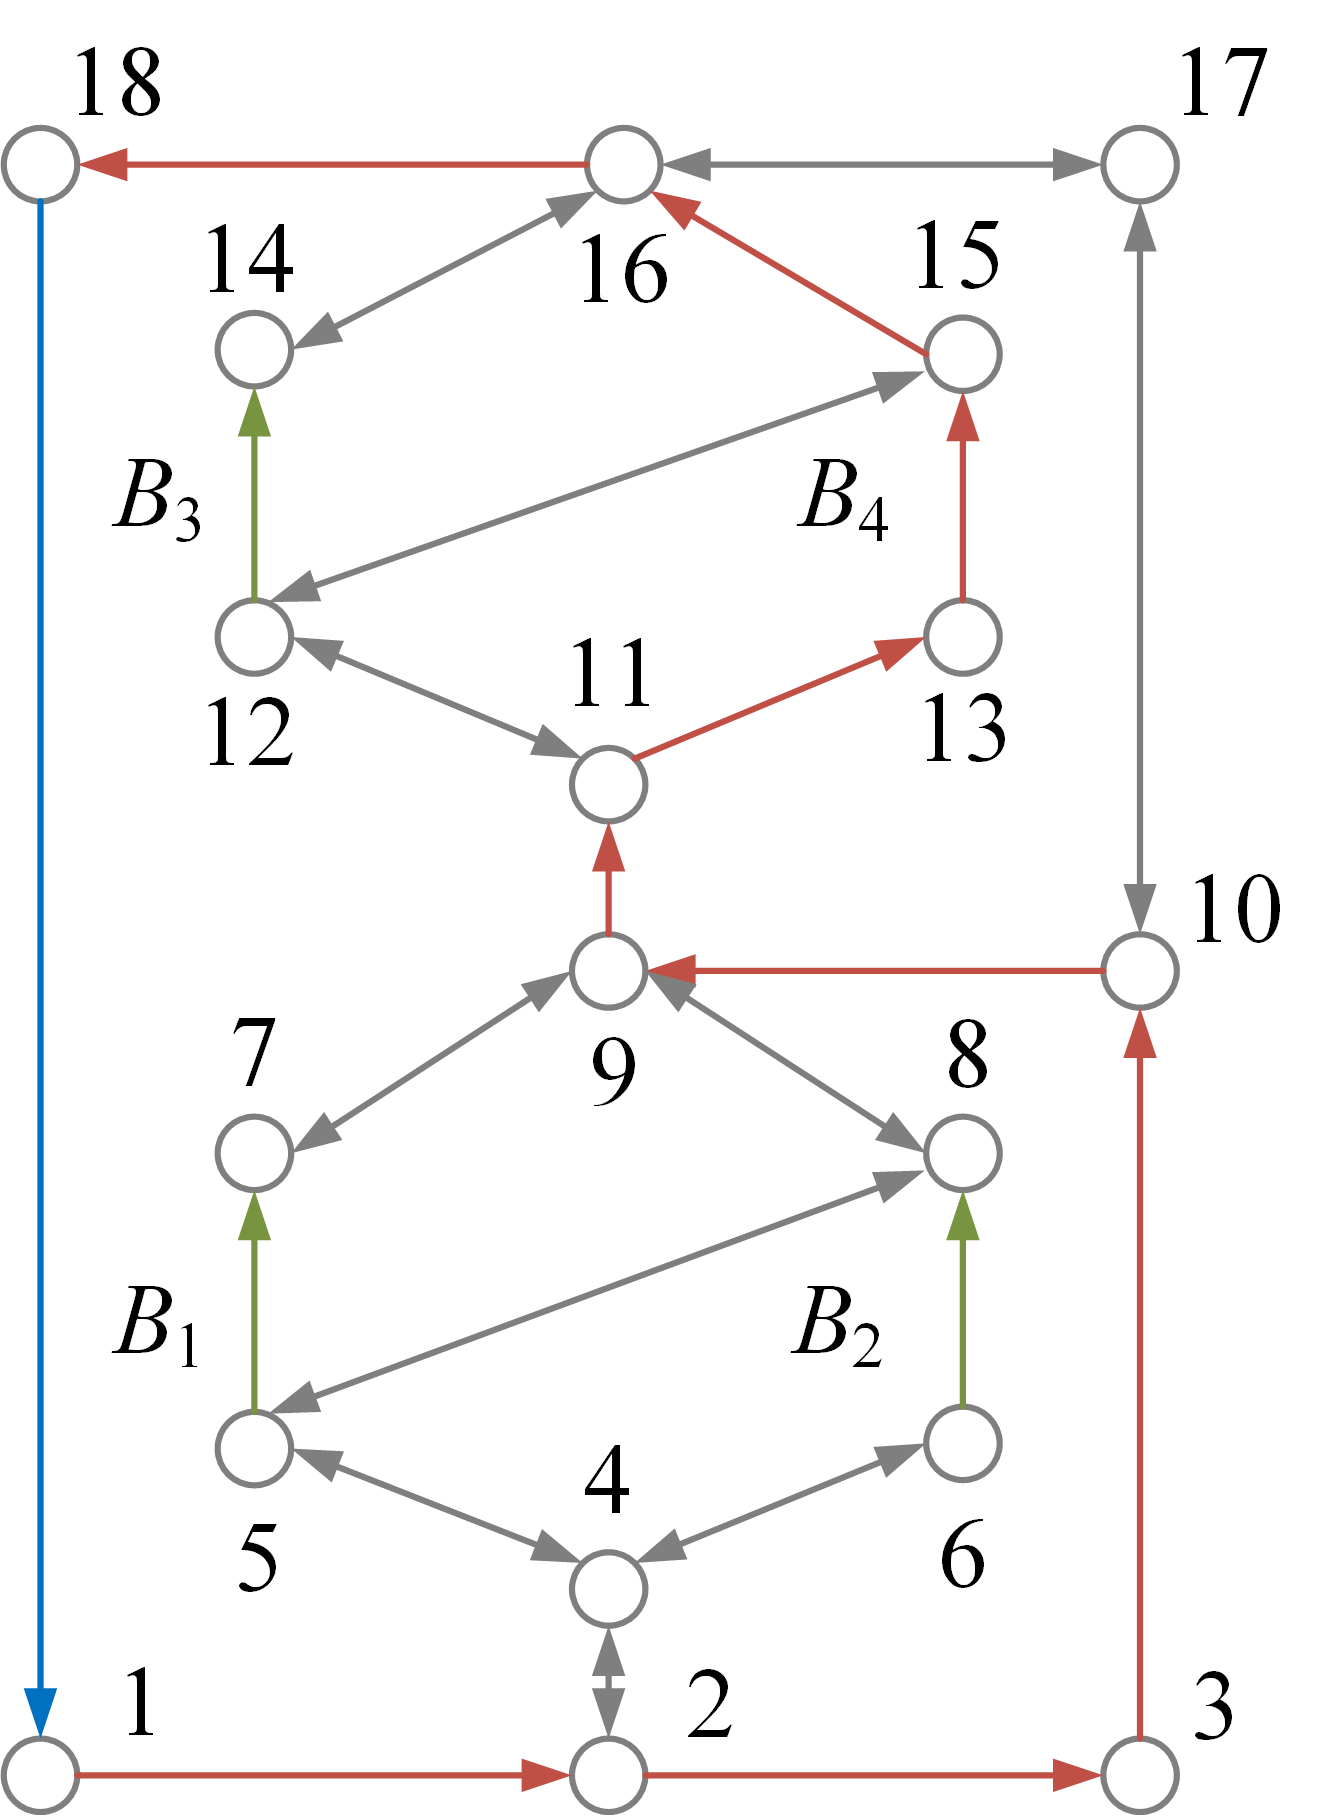
\includegraphics[width=\textwidth]{../attachments/ef-sp4.png}
        \caption{}
        \label{fig:sp4}
    \end{subfigure}
    \caption{
        The $SP$s of battery cell (a)$B_1$ (b)$B_2$ (c)$B_3$ (d)$B_4$ in the new structure's topological model, which is highlighted in red.
        }
\end{figure}

\begin{table}[htbp]
  \centering
    \caption{MAC Calculating result of the output current $I_o$, battery current $\bm{I}_b$ and ratio $\eta$ in the structure combining Lawson et al.\cite{lawsonSoftwareConfigurableBattery2012} and Visairo et al.\cite{visairoReconfigurableBatteryPack2008} with 4 battery cells and 19 switches.}
    \begin{tabular}{cc}
    \toprule
        % Structure & combining Lawson et al.\cite{lawsonSoftwareConfigurableBattery2012} and Visairo et al.\cite{visairoReconfigurableBatteryPack2008} with 4 battery cells and 19 switches  \\
        Structure & 4 battery cells and 19 switches  \\
    \midrule
    Switch ON & 1,3,5,6,8,9,10,12,18,19 \\
    $\bm{X}_s$ & $\diag(1,0,1,0,1,1,0,1,1,1,0,1,0,0,0,0,0,1,1)$ \\
    \midrule
        $I_o$ & $2u_b/(2R_o+r_b)$ \\
        $\bm{I}_b$ & $[u_b/(2R_o+r_b),u_b/(2R_o+r_b),0,0]$ \\
        $\eta$     & 2 \\
    \bottomrule
    \end{tabular}%
  \label{tab:find_mac}%
\end{table}%

\begin{figure}[htbp]
    \centering
    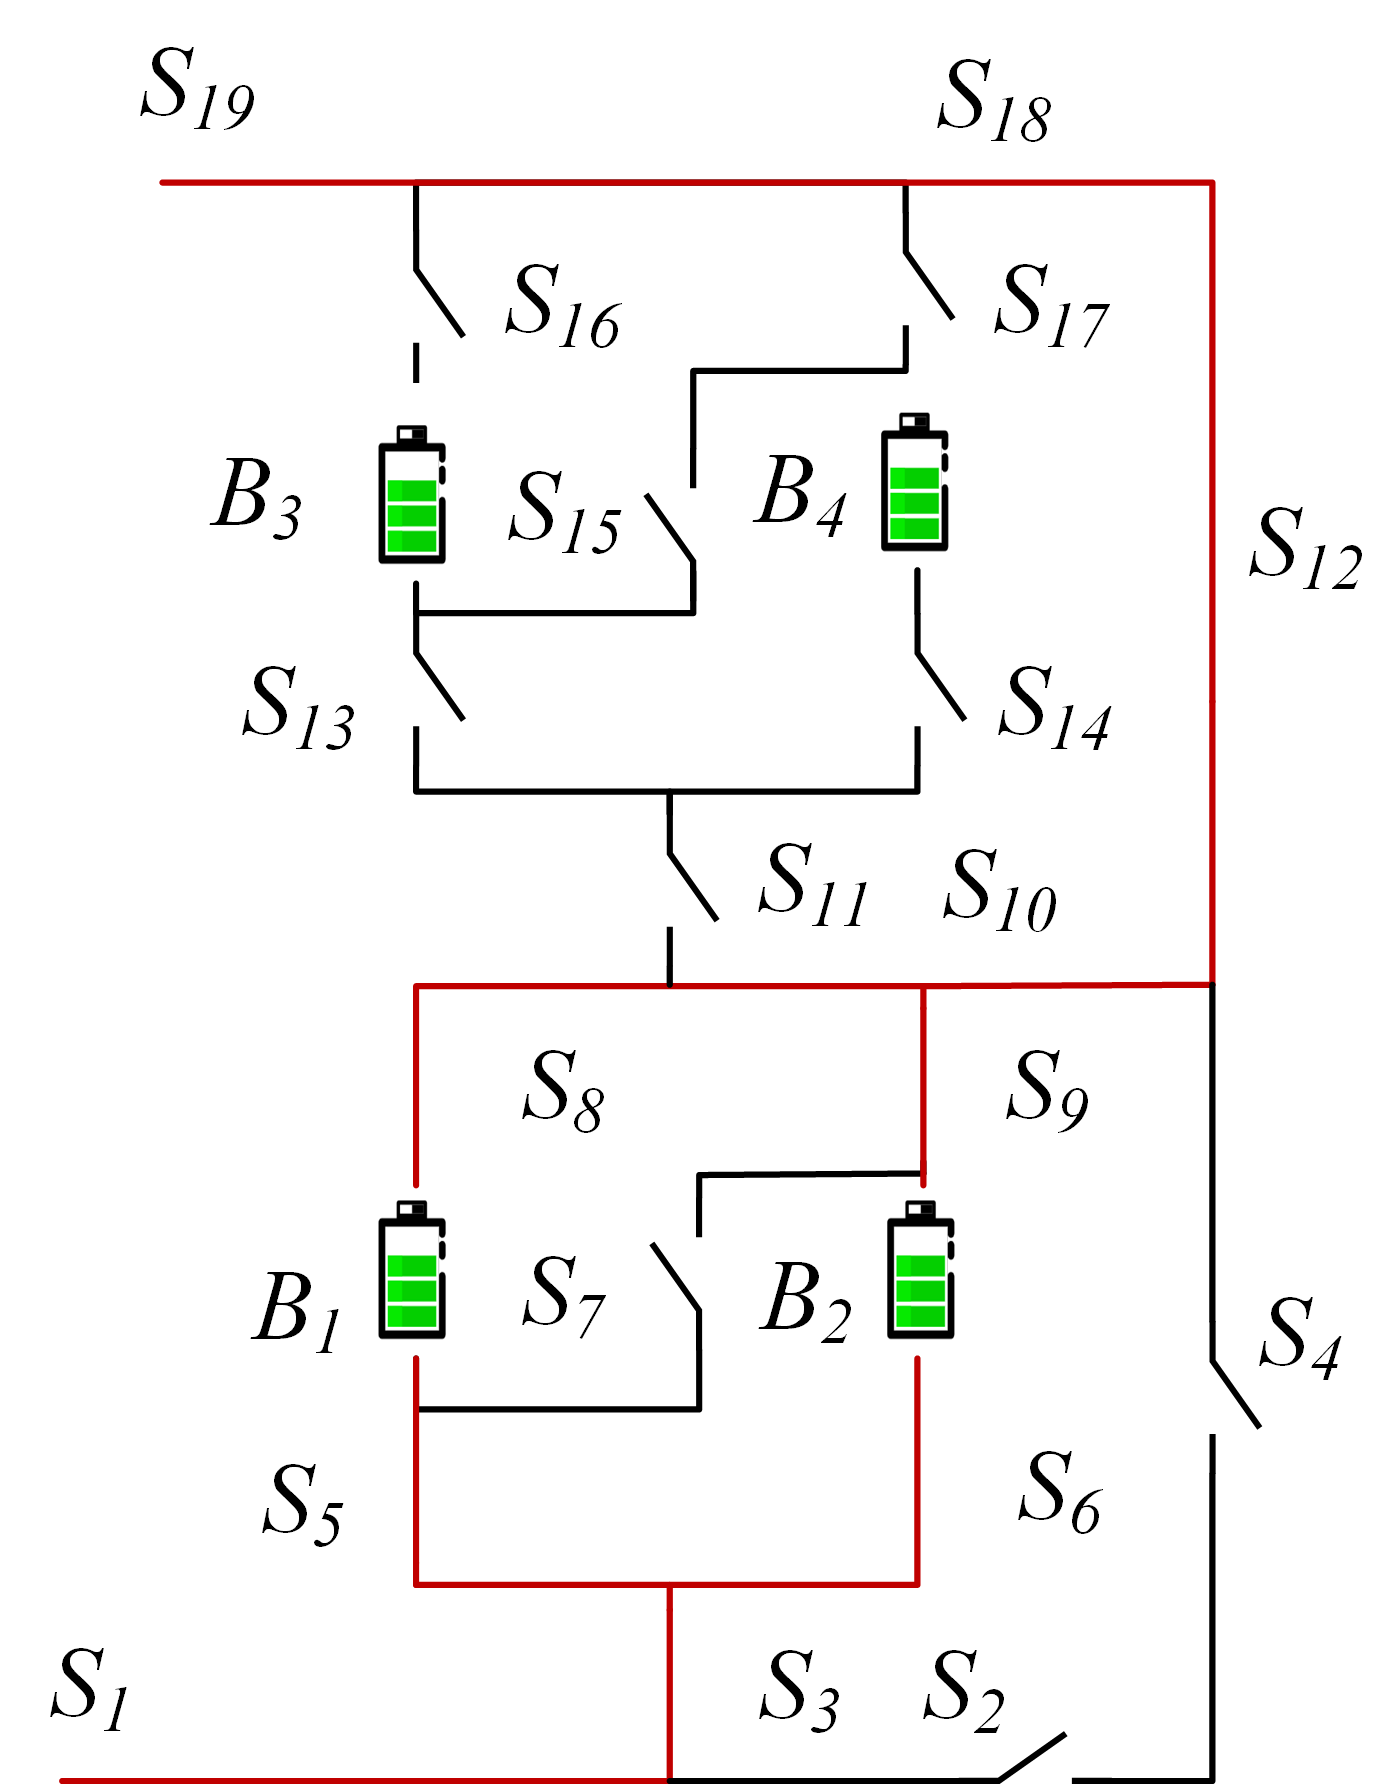
\includegraphics[width=0.5\textwidth]{../attachments/ef-mac.png}
    \caption{
        The finally calculation result of MAC for the new structure with four battery cells and 19 switches.
        The red lines represent the branches through which the current flows, and the switches on these branches are ON. 
        In this situation, the RBS outputs MAC to the outside, which is $\eta=2$.
    }\label{fig:ef-mac}
\end{figure}

\subsection{Discussion}

The correctness of the results shown in Fig. \ref{fig:ef-mac} is obvious. 
When B1 and B2 or B3 and B4 are connected in parallel, the RBS can output the maximum current, which is $\eta=2$, i.e. twice the current output of a single battery in RBS.
While adding more batteries to the main circuit can only form a series structure and will not improve the MAC.
It is worth noting that when solving for MAC, $\eta$ is used as the objective function instead of $I_o$, which makes the result of MAC more reasonable. 
According to the results shown in Tab. \ref{tab:find_mac}, $I_o$ and $\bm{I}_b$ are affected by the equivalent resistance $R_o$ of external electrical appliance, the battery's electromotive force $u_b$, and internal resistance $r_b$. 
This means that if $I_o$ is used as the objective function, even for the same RBS structure, the MAC result and corresponding switch state could be changed due to different external electrical appliances. 
This increases the difficulty and uncertainty in RBS structure design. 
On the contrary, by using $\eta$ as the objective function, which dividing $I_o$ and $\max\bm{I}_b$, the influence of these factors on the results is eliminated, as shown in Tabs. \ref{tab:given_x} and \ref{tab:find_mac}.
$\eta$ only reflects the maximum output current capability of the RBS structure.
Assuming that the maximum allowed current of battery cells in the RBS is $I_m$, the maximum output current of the RBS structure can be calculated as $\eta I_m$ by calculating the $\eta$ of the structure. 
Therefore, compared to $I_o$, $\eta$ is more suitable for structure design. 
Most of the currently proposed RBS structures\cite{ciNovelDesignAdaptive2007,alahmadBatterySwitchArray2008,kimDependableEfficientScalable2010b,kimBalancedReconfigurationStorage2011a,taesickimSeriesconnectedSelfreconfigurableMulticell2012a,6843711} have simple topological characteristics, and the calculation of MACs are relatively simple, even intuitive.
However, when complex and flexible structures need to be designed for application scenarios such as equalization or isolation of specific battery cells, the estimation of MAC will become complex and complicated. 
The method proposed in this paper can effectively solve any RBS structure and estimate MAC universally, paving the way for the structure design of more complex and flexible RBSs.

% 对比Tab. 1和 Tab. 2,可以发现,对于这两种开关状态 $\bm{X}_s$,在电阻和电动势相同的情况下,前者的Io更大。
% 这主要是由于在Tab. 1的情形下,四个电池以两并两串的形式接入主电路,提供了更多的电动势。
% 相应的,每个电池的电流也更大。
% 此时,如果仅使用 Io 作为目标函数,则  () #TODO:讨论怎么说

When the RBS has isolated battery cells, the original topology of the structure is altered. 
However, the method proposed in this paper can still be used to calculate the MAC of the new structure. 
The MAC after the isolation operation can be obtained by calculating the new structure following the procedures described in the previous subsection.
During the calculation process, the isolated battery cell(s) do not participate in the calculation, i.e., their nodes, edges, and $SP$s are not considered. 
The MACs under various isolated battery cell(s) are calculated on the structures proposed by Lawson et al. (Fig. \ref{fig:arch-e}), Visairo et al. (Fig. \ref{fig:arch-f}), and the new structure that integrates the previous two structures (Fig. \ref{fig:ef-topo}), as shown in Fig. \ref{fig:isolated_mac}. 
For the structure proposed by Lawson et al., the MAC remains the same as that without isolated battery cells, i.e., $\eta=1$, when the number of isolated battery cells increases, until all the cells in the RBS are isolated.
For the structure proposed by Visairo et al., the MAC decreases as the number of isolated battery cells increases, until $\eta=0$.
While the new structure has two cases of isolating two cells, one is to isolate two cells within the same substructure, in which case $\eta=2$; the other is to isolate one cell in each of the two substructures, in which case $\eta=1$. 
Overall, the MAC of the new structure is positioned between the structures proposed by Lawson et al. and Visairo et al..
It can be seen that the MAC of the structure in Fig. \ref{fig:arch-e} is the most stable, and the structure has advantages in isolation and redundancy backup, but its MAC is the smallest. 
The structure proposed shown by Fig. \ref{fig:arch-f} can output the largest MAC but is susceptible to the number of isolated battery cells. 
However, the structure proposed by this paper has certain advantages in both aspects, being insensitive to the number of isolated battery cells while simultaneously achieving a larger MAC.

\begin{figure}[htbp]
    \centering
    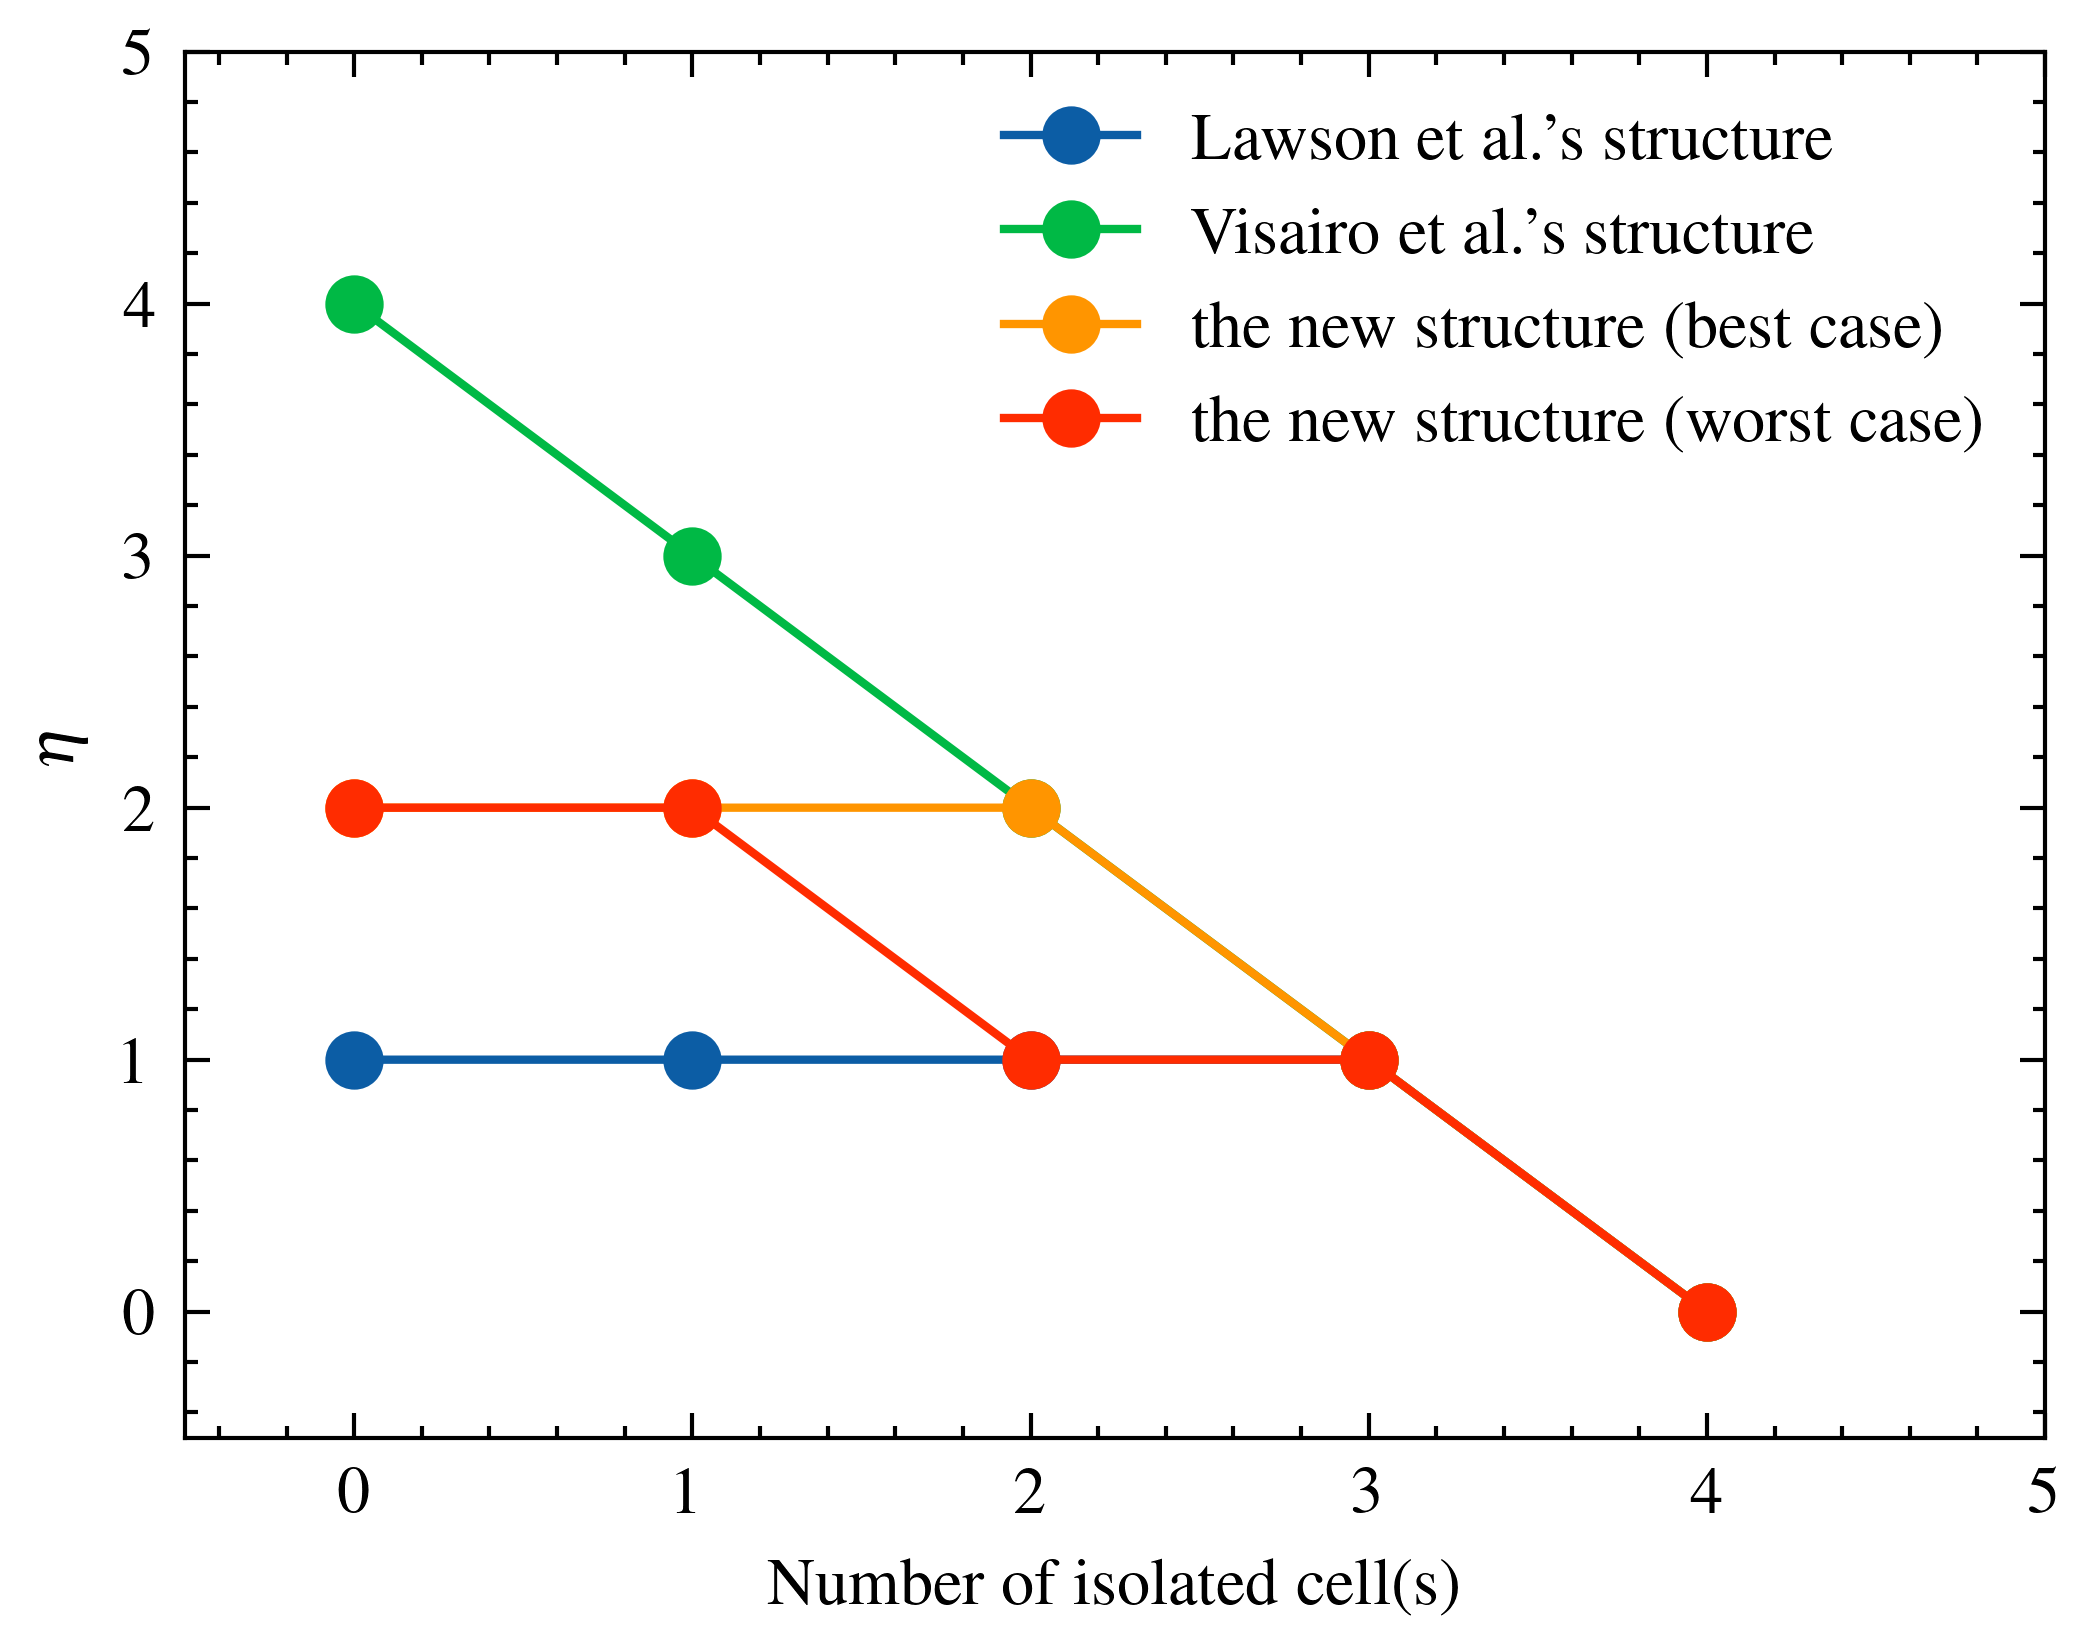
\includegraphics[width=0.8\textwidth]{../attachments/isolated_mac.png}
    \caption{
        The variation of MAC with the number of isolated battery cells for different RBS structures, including the structure proposed by Lawson et al., Visairo et al. , and the new structure in this paper.
    }\label{fig:isolated_mac}
\end{figure}

\section{Conclusion}

This paper firstly proposes a method to calculation the MAC of RBS according to its architecture. 
To find the circuit in RBS that enable the MAC, a greedy strategy incorporate with the topologic model is developed to. 
The effectiveness of proposed method is tested on a more complex RBS structure based on two proposed structure.
This work presents an effective approach to evaluate the MAC of RBS, which is essential for design and management of the RBS. 
Future research could focus on developing new performance indicators for evaluating RBS performance using the currents and voltages obtained by this method, as well as modifying the equivalent model of the battery to enable more accurate simulations of RBS, including transient analysis.

% \section{Appendix}
% \begin{algorithm}
%     \caption{Get the max available currents of a certain RBS}\label{alg:eta_RBS}
%     \KwData{Directed graph model $G(V,E)$ of the RBS}
%     \KwResult{$\max \eta$}
%     \For{$i \in E_b$}{
%         $P_i \leftarrow \{path| \text{starts at $v_1$ and ends at $v_n$} \}$\;
%         $SP_i \leftarrow p_i \text{ which has the minimum}~\omega(p_i)~\text{among all}~p_i \in P_i. $
%     }
%     get $\bm{A}$ by Equation \ref{eq:A}\;
%     \While{not yet determine $\max \eta$ }
%     {
%         $N_{sel} \leftarrow \text{number of selected $SP$s calculated by dichotomy}$\;
%         $C_b    \leftarrow \text{set of all combinations of $N_{sel} $~batteries from $N_b$}$\;
%         \For{$c_b \in C_b$}{
%             $\bm{x}_s \leftarrow \text{list of all switches' state: $x_s[j]=1$ if $ j \in \bigcup_{i\in c_b}SP_i $ else 0}$\;
%             $\bm{X} \leftarrow diag[1,1,\cdots,1,\bm{x}_s] $\;
%             get $\bm{Y}_n$ by Equation \ref{eq:Yn}\;
%             \eIf{$\bm{Y}_n$ is invertible}{
%             }{construct an effective solution}
%             get $I_o$ by Equation \ref{eq:I_o}\;
%             get $\bm{I}_b$ by Equation \ref{eq:I_b}\;
%             \eIf{$\max(\bm{I}_b)\leq I_m$}{
%                 $\eta \leftarrow I_o/\max(\bm{I}_b)$\;
%             }{break}
%         }
%     }
% \end{algorithm}

\bibliographystyle{ieeetr}
\bibliography{my_ref}

\end{document}
